\section{问题四的模型建立与求解}

按照``模型建立 $\to$ 模型求解 $\to$ 模型验证''的流程组织本节。问题四
要求：（1）基于附件 C 把开源模型能力提升分解为规模扩张与非规模技术
进步的贡献；（2）在算力增长放缓情景下预测未来 12/24 个月能力前沿并给不确定
区间；（3）完成至少一项基于 C8 的逐任务聚合分析。数据侧：C1/C2 为排行榜
（4576 条，6 维平均分 + 参数量 + 提交日期 + 许可证），C3 为扩展时序
（2019--2025），C4 为 Epoch 模型库（含算力、参数、开源权重标记），C5/C6
为 Loss--Benchmark 桥接，C7 为架构元数据，C8 为逐任务明细。

\subsection{模型建立}

\subsubsection{综合能力度量与数据口径}

\textbf{能力度量}：采用 C1 排行榜 6 维平均分 $S\in[0,100]$（IFEval、BBH、
MATH-Lvl5、GPQA、MUSR、MMLU-Pro 的平均）。该指标覆盖指令遵循、推理、数学、
科学问答与多步推理，作为综合能力代理变量。

\textbf{开源筛选口径}：以 C1 的 \texttt{Hub License} 含开源许可词
（apache/mit/bsd/llama/gemma/cc-by 等）为主判据，并交叉核对 C4 的
``Open model weights?'' 标记；筛选出开源模型 2496/4564 条，后续前沿分析
仅用开源子集，避免闭源模型（如 GPT 系列）的能力虚高与数据泄露。

\textbf{模型类型区分}：C1 的 \texttt{Type} 字段将模型分为 pretrained
（$n=275$）、chat/RLHF/DPO/IFT（$n=718$）、域特定微调（$n=1785$）与
基座合并（$n=1724$）等。按题意区分 pretrained 与 chat/finetuned，独立
复算（v80）：主链路全开源子集（$n=2493$）$b_N=0.364$、$b_T=0.089$、规模
贡献 83.7\%；\textbf{剔除 chat 与域微调子集}后（保留 pretrained/持续预训练/
基座合并等非对齐微调类型，$n=920$）$b_N=0.365$、$b_T=0.068$、规模贡献
升至 87.0\%——
``规模主导''对模型类型口径\textbf{稳健}；而纯 pretrained 子集（$n=239$，
样本稀疏）时间项 $b_T\approx-0.03$（年度趋势近似为零），chat 子集
（$n=459$）$b_T=0.129$——前沿分解中的``非规模技术''成分主要来自对齐/
微调通道的能力增益，纯预训练基座的年度技术进展有限。

\textbf{时间轴口径}：采用排行榜的\textbf{提交日期}（Submission Date）作为
时间轴——排行榜以提交即测为准，避免发布/版本日期在提交前多次迭代带来的
时间歧义（C4 的发布日期仅用于交叉核对开源权重标记）。

\textbf{开源子集对全量前沿的近似性核验}（图 \ref{fig:p4_opengap}）：按季度
对比开源前沿（开源行平均分最大值）与全量前沿：2024Q2 比值为 0.87，2024Q3
与 2025Q1 开源模型即为全量领跑者（比值 1.00），2024Q4 为 0.91——四个季度
中两个季度开源前沿\textbf{追平}全量前沿，平均比值约 0.95。开源子集作为
``前沿代表''的近似误差有限，且未系统性低估；这一核验也表明开源策略
（开放权重生态）在能力前沿上具备持续竞争力。

\begin{figure}[htbp]
\centering
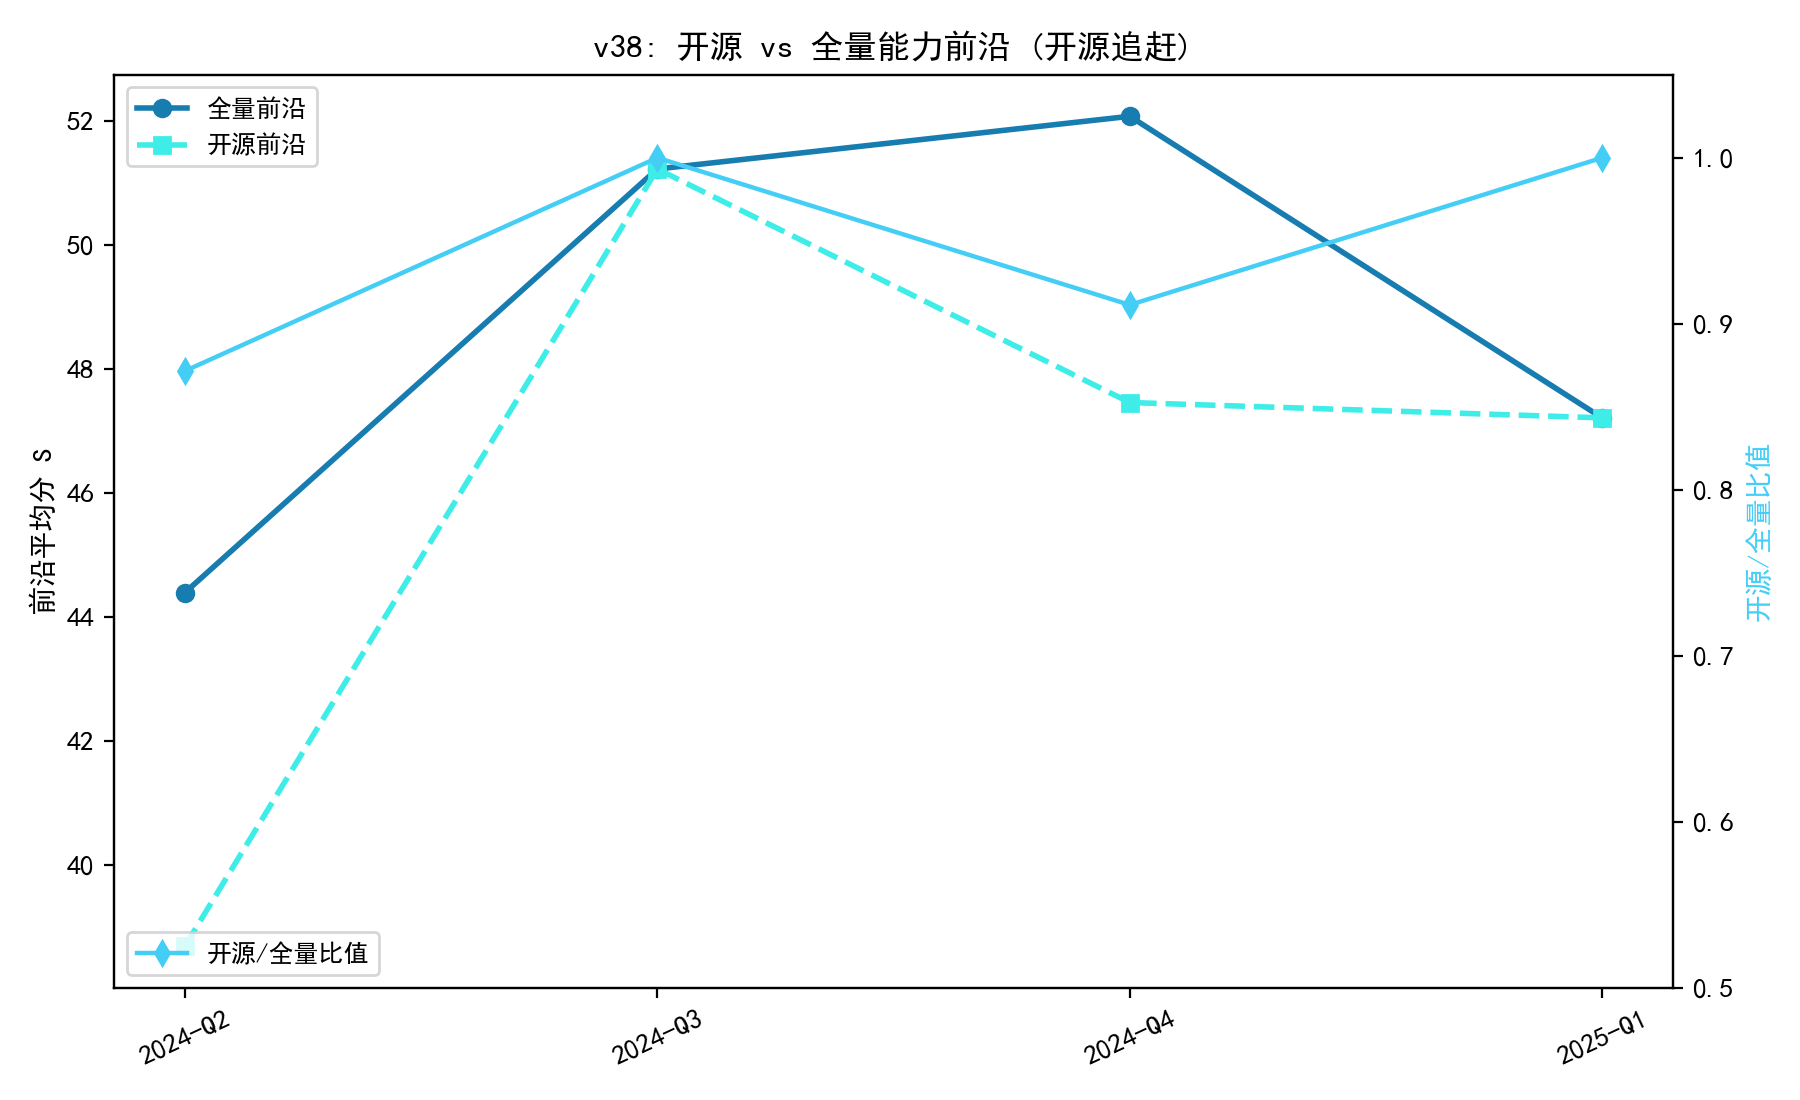
\includegraphics[width=0.82\textwidth]{figures/v38_p4_open_gap.png}
\caption{开源 vs 全量能力前沿：开源在 2024Q3/2025Q1 追平全量领跑。}
\label{fig:p4_opengap}
\end{figure}

\textbf{差距的规模段分解}（图 \ref{fig:p4_opeseg}）：把开/闭源差距按
参数规模分桶，中位分比值（open/closed）：$0.3$--$1$B 段 0.93$\to$0.89
（开源落后约 10\%）；$1$--$3$B 段 0.79$\to$1.13（\textbf{开源反超}）；
$3$--$10$B 段长期持平（约 1.00）；$10$--$30$B 段 1.35$\to$0.82$\to$1.07
（波动后趋平）；$30$--$100$B 段 0.88$\to$0.98（追赶中，样本较稀）。
\textbf{开源追赶分规模段}：中段（$1$--$10$B）已基本完成/接近，两端
（最小端与头部大模型）仍落后约 10\%——v38 的平均比值 0.95 在此分解为
``中段持平 + 两端滞后''的结构。

\begin{figure}[htbp]
\centering
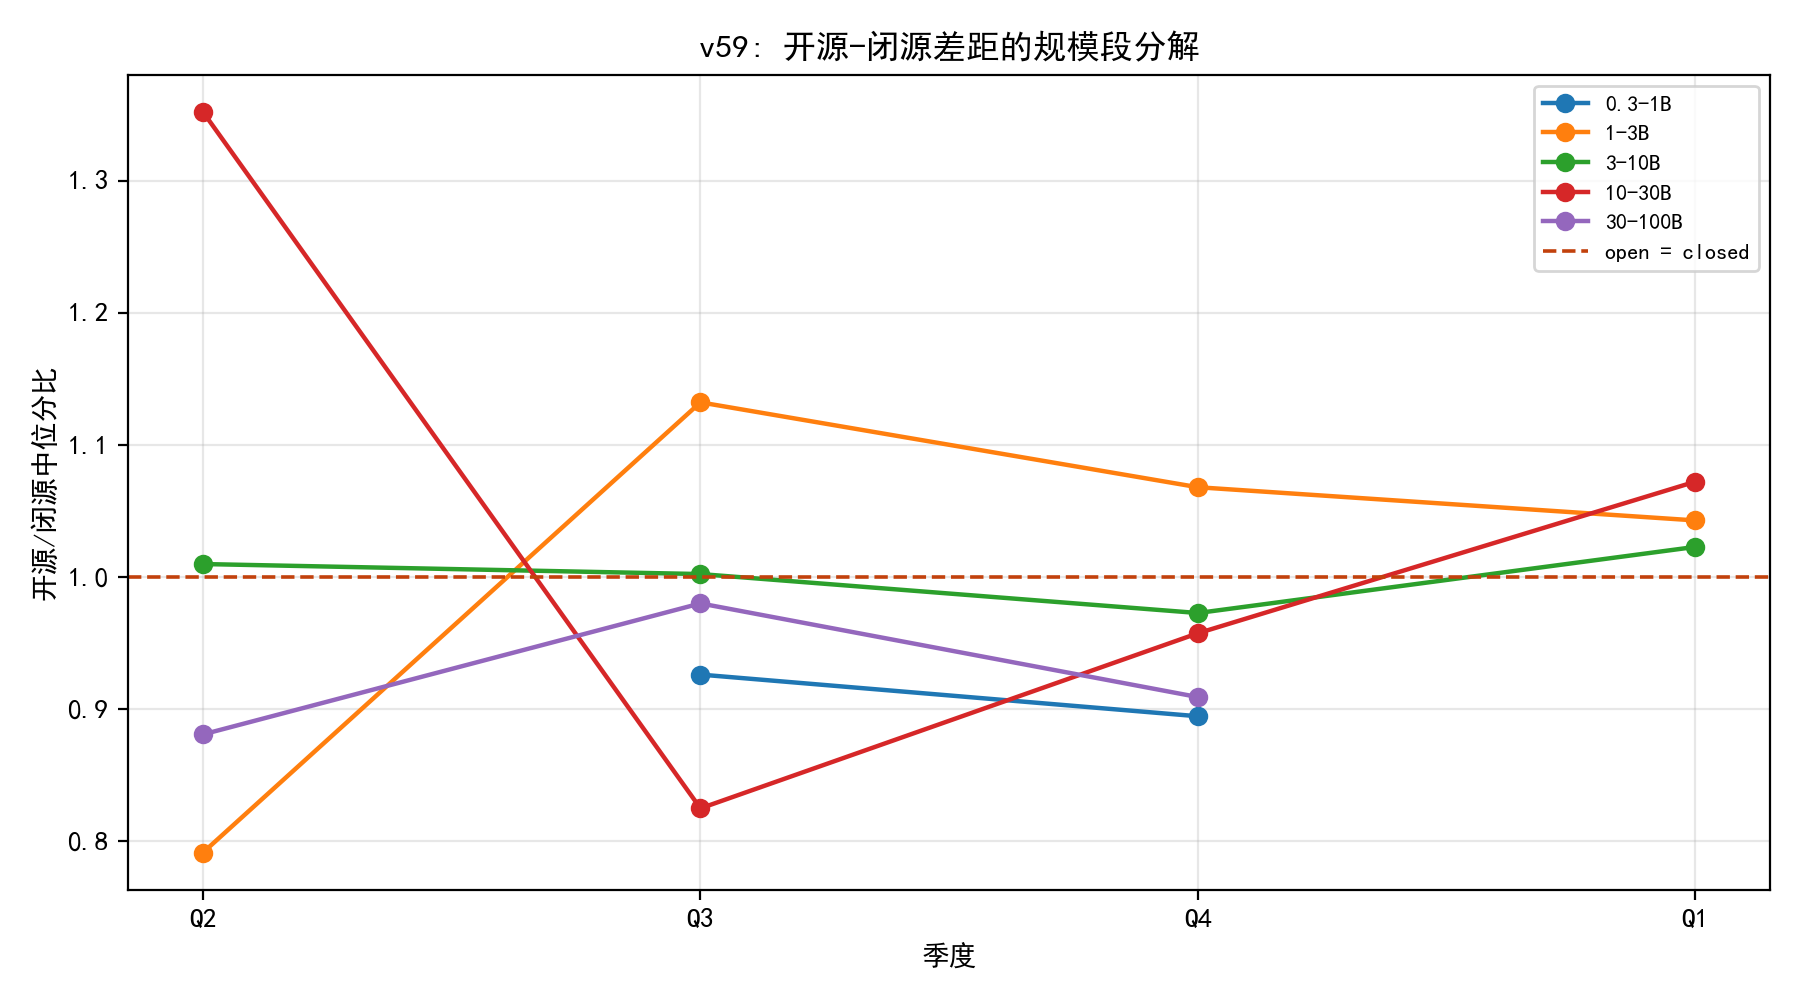
\includegraphics[width=0.85\textwidth]{figures/v59_p4_open_seg.png}
\caption{开源--闭源差距的规模段分解：中段持平、两端滞后约 10\%。}
\label{fig:p4_opeseg}
\end{figure}

\textbf{开源前沿的家族竞争动态}（图 \ref{fig:p4_family}）：按季度识别开源
领跑家族：2024Q2 为 Llama（38.7），Q3 与 2025Q1 由其他家族领跑（51.2/47.2，
Qwen 连续居于次席），Q4 为 Qwen（47.5）。前 5 高分模型家族的 HHI 从 2024Q2
的 1.00（单家垄断）降至 Q3--Q4 的 0.52、2025Q1 的 0.68，季度内活跃家族数
9--11——开源前沿的竞争从``一家独大''走向``多家族并立''，且 Qwen 持续
占据领跑梯队，家族更替快于单一模型的换代周期。

\begin{figure}[htbp]
\centering
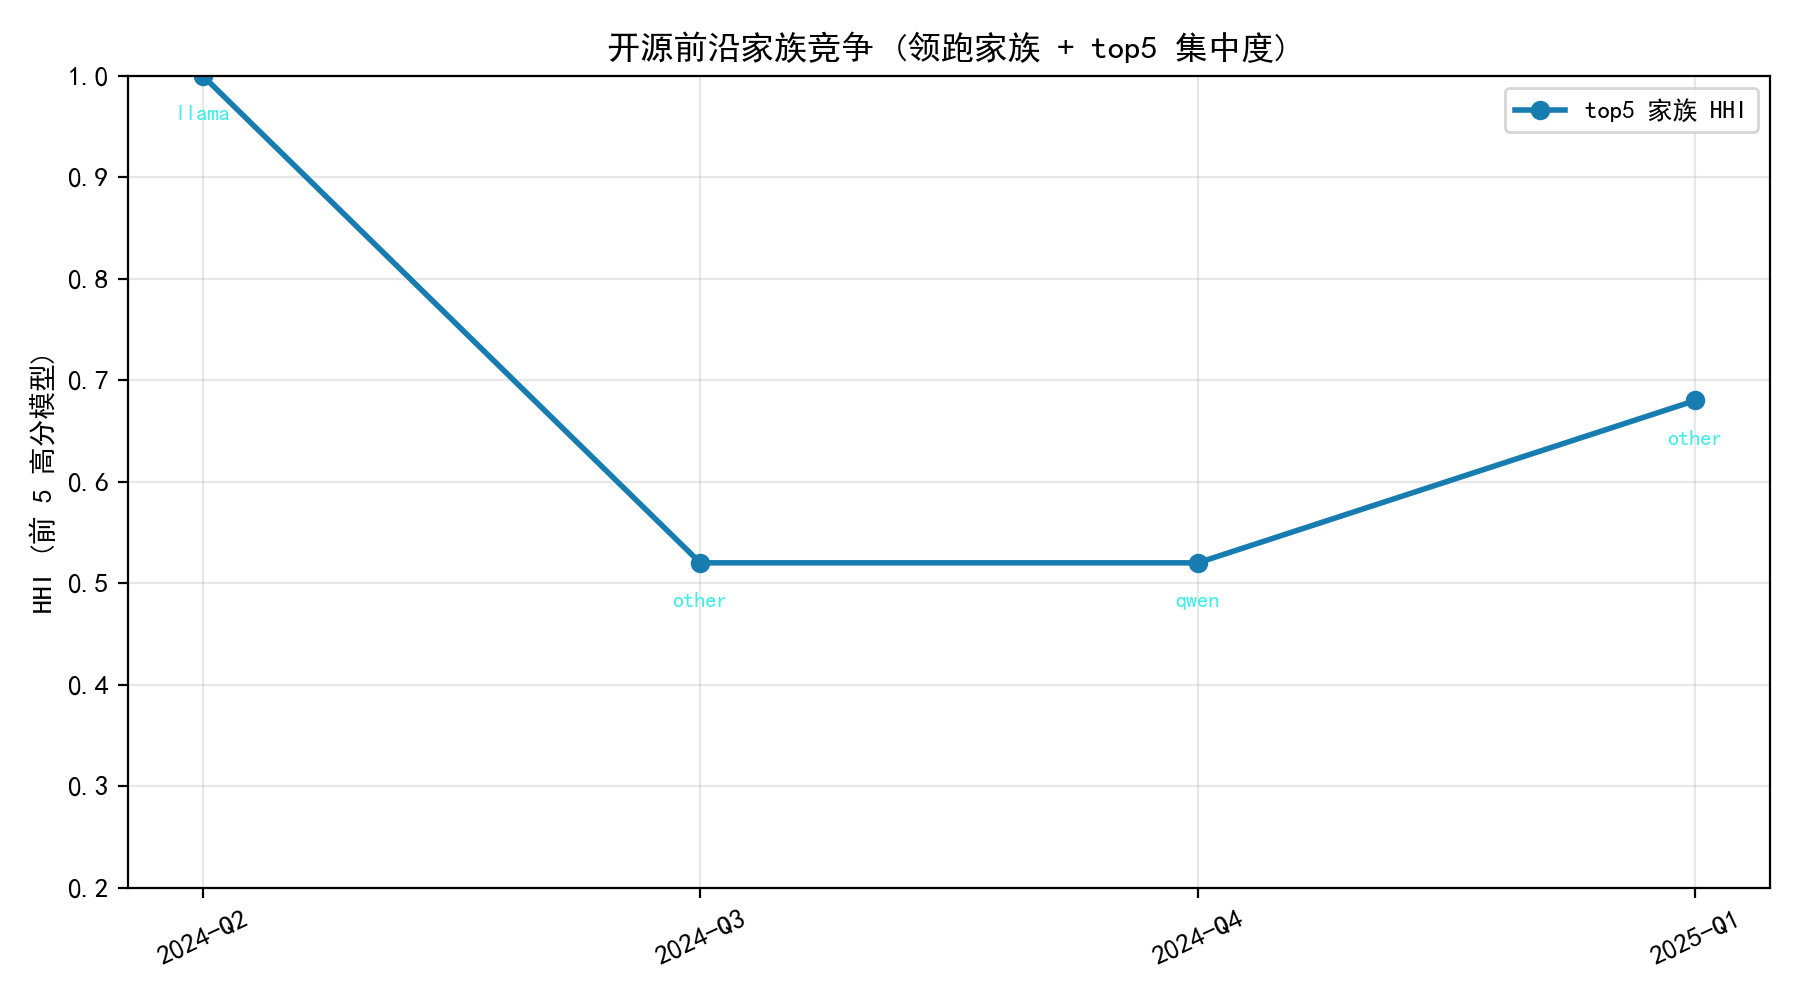
\includegraphics[width=0.8\textwidth]{figures/v42_p4_family_dyn.png}
\caption{开源前沿家族竞争：领跑家族轮替与 top5 集中度（HHI）。}
\label{fig:p4_family}
\end{figure}

\textbf{追赶时间的外推预测}（图 \ref{fig:p4_catchup}）：v42 给出的是
\textbf{历史轮替}（领跑身份季度间更迭），这里用 2025-03 家族 90 分位与
对数线性增速做\textbf{前向外推}：领跑者为 Qwen（43.1，月增速 +0.057）；
仅 ``other'' 聚合类（41.9，差距 3\%）预计约 6 个月追平、Mistral（38.1）
需约 137 个月（11 年，仅略快）；Phi（39.9）、Gemma（21.6）增速不足，
\textbf{Llama（30.5）月增速仅 +0.004（年化 +0.04，近乎停滞）}、Yi
（12.7）甚至负增长（$-1.39$/年），均判定为``永不''收敛（当前增速差
持续）。合起来：近期多强轮替（v42），\textbf{外推下收敛到 Qwen 单极 +
其余固定差距}——增速结构比领跑身份更能预示格局走向。（注意：90 分位
增速含发布节奏噪声，``永不''指当前增速差延续的推演；对增速结构做
模型层 Bootstrap（300 次）后，确定性外推中可追赶的 other/Mistral 两族
``永不收敛''的样本占比仍达 53\%--65\%，追赶时间 90\% 区间分别宽达
$1.1$--$63.9$、$4.4$--$213.5$ 个月——外推不确定性显著，结论仅在增速
结构维持假设下成立。）

\begin{figure}[htbp]
\centering
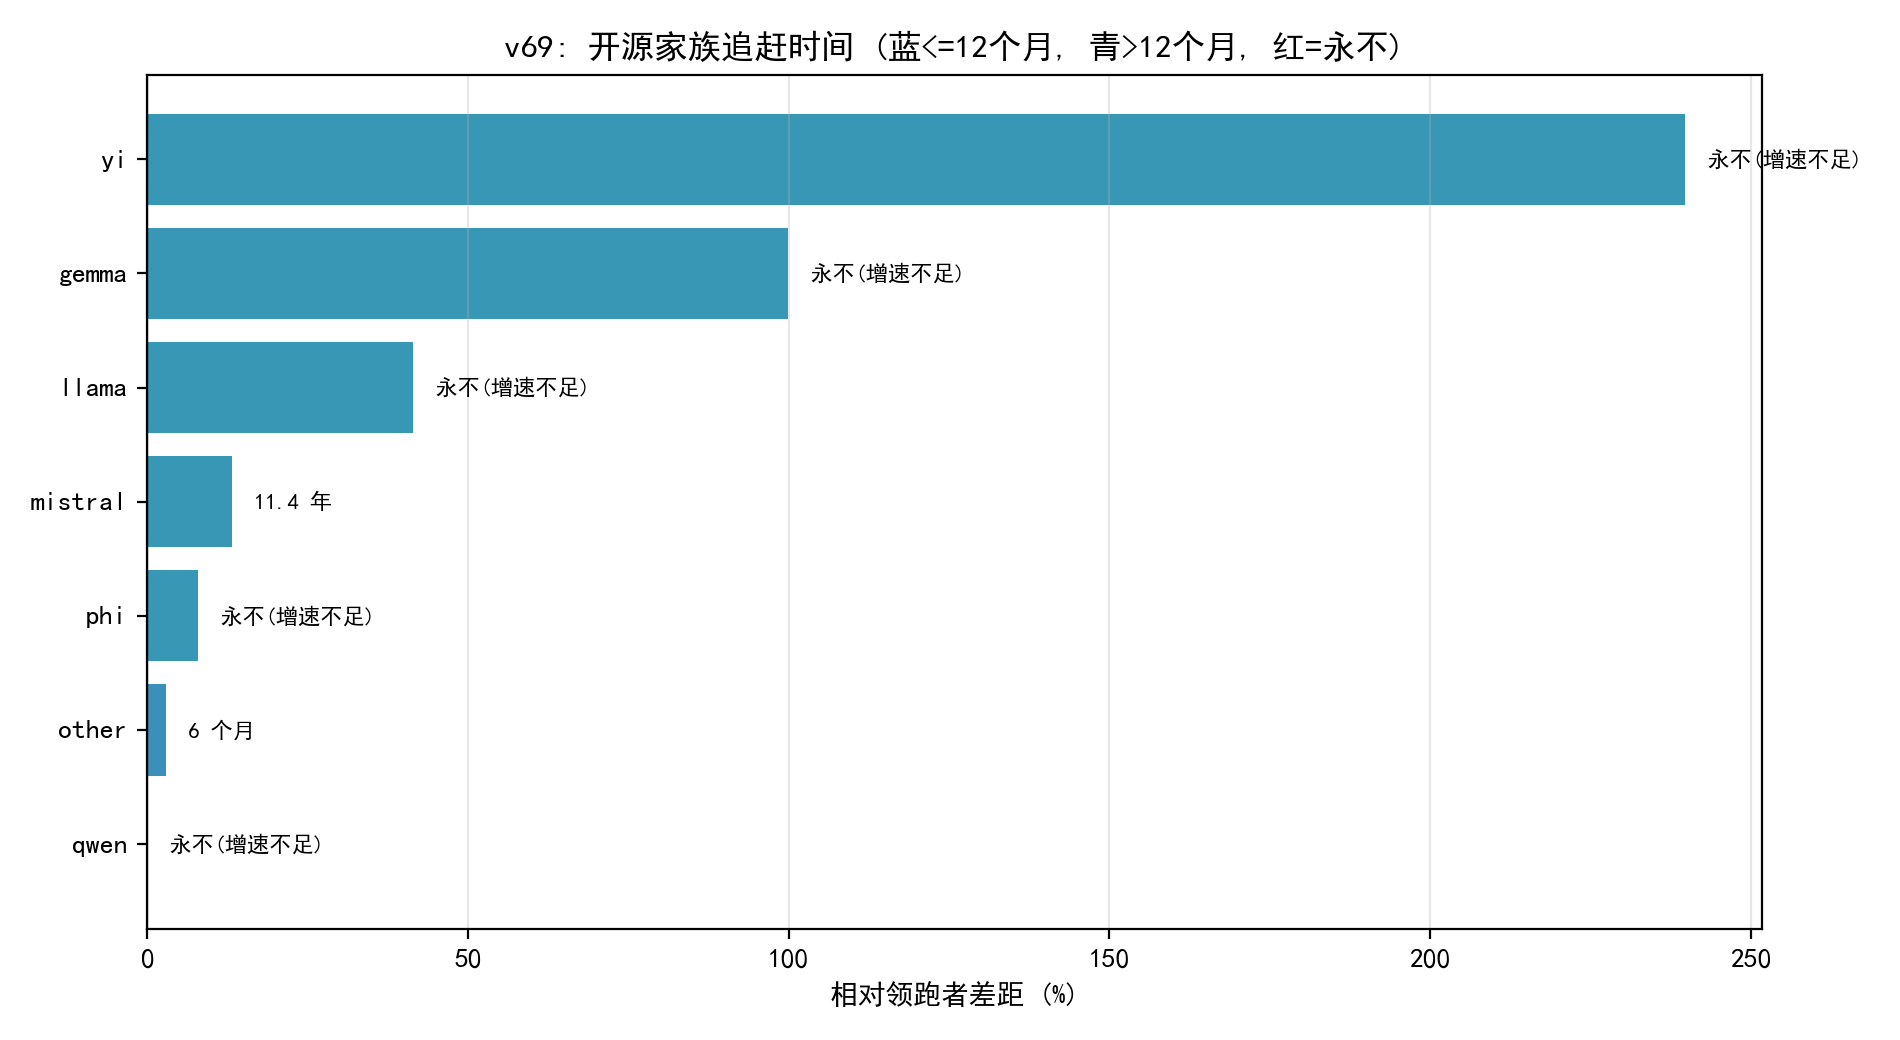
\includegraphics[width=0.85\textwidth]{figures/v69_p4_catchup.png}
\caption{家族追赶时间：仅 other 可短期追平，Llama 近乎停滞。}
\label{fig:p4_catchup}
\end{figure}

\textbf{时间轴口径}：以 C1 的提交日期（Submission Date）作为年份依据；
C3 的历史前沿（2019--2021）作为补充背景，取累计最大值以保证前沿单调不降
（2020 年出现 50.0 的孤立高值、2021 回落，属半合成扩展数据，取累计口径
规避该噪声）。

\subsubsection{前沿能力模型}

对开源模型样本建立 90\% 分位数回归：
\begin{equation}
\ln S = c + b_N \ln N + b_T t,
\label{eq:frontier}
\end{equation}
其中 $t$ 为以 2022 年为 0 的年份。分位数回归（线性规划形式，Koenker--
Bassett 精确解）对前沿点稳健，比均值回归更能刻画``能力前沿''。拟合结果
（$n=2493$）：
\begin{equation}
c=2.481,\qquad b_N=0.364,\qquad b_T=0.089.
\label{eq:frontier_fit}
\end{equation}
解释：$b_N=0.364$ 表示参数每翻倍、前沿平均分（对数尺度）提升
$\ln2\times0.364\approx0.252$，对应水平增幅约 $28.7\%$；$b_T=0.089$
表示即使参数不变，每年前沿
整体上移约 9\%——这就是非规模技术进步（算法、对齐、数据组织、工程优化）的
量化体现。作为对照，普通最小二乘会得到 $b_T=0.20$（高估技术增速），
Huber 稳健回归 $b_T=0.24$（v79 复算），均因受大量非前沿样本拖累而失真；分位数回归
专门追踪前沿点，取值最可信。对参数做 300 次样本自助（在 $\tau=0.9$ 的
线性规划分位数回归上重抽）得 90\% 置信区间：$b_N\in[0.347,0.378]$、
$b_T\in[0.068,0.103]$，均显著异于 0；对应规模贡献占比区间约为
81\%--87\%，``规模主导''结论在参数不确定性下稳健。

\textbf{跨框架一致性核验}（图 \ref{fig:p4_qrfw}）：为保证分位数前沿结论
不依赖统计实现，用五个相互独立的框架复算同一 $\tau=0.9$ 回归——线性规划
精确解（HiGHS，主链路）、statsmodels QuantReg、sklearn
QuantileRegressor（$\alpha=0$）、L-BFGS-B 直接极小化 pinball 损失与 Adam
梯度下降。结果：\textbf{五框架复现同一系数}——$c_0=2.481$、$b_N=0.364$、
$b_T=0.089$（相对极差：$c_0$ 为 $4\times10^{-3}\%$、$b_N$ 为
$2\times10^{-2}\%$、$b_T$ 为 $3\times10^{-1}\%$——后者来自 Adam 梯度下降
在有限步数下的微小未收敛，其余四框架逐位一致），pinball 目标值在
LP/statsmodels/sklearn/L-BFGS-B 四框架一致到 6 位小数（135.95035；
Adam 相差 $\le2\times10^{-3}$），$n=2493$ 个样本上的预测最大跨框架差异
仅 $1.0\times10^{-3}$。代入
增长核算式 (\ref{eq:growthacc})（$g_N=1.251$），五个框架给出的规模贡献
占比\textbf{全部为 $83.66\%$}（差异 $\le4\times10^{-4}$）。跨
scipy/statsmodels/sklearn/torch 四个统计生态的独立实现收敛到同一前沿，
证明\textbf{前沿系数与规模/非规模分解对估计器实现数值稳健}。

\begin{figure}[htbp]
\centering
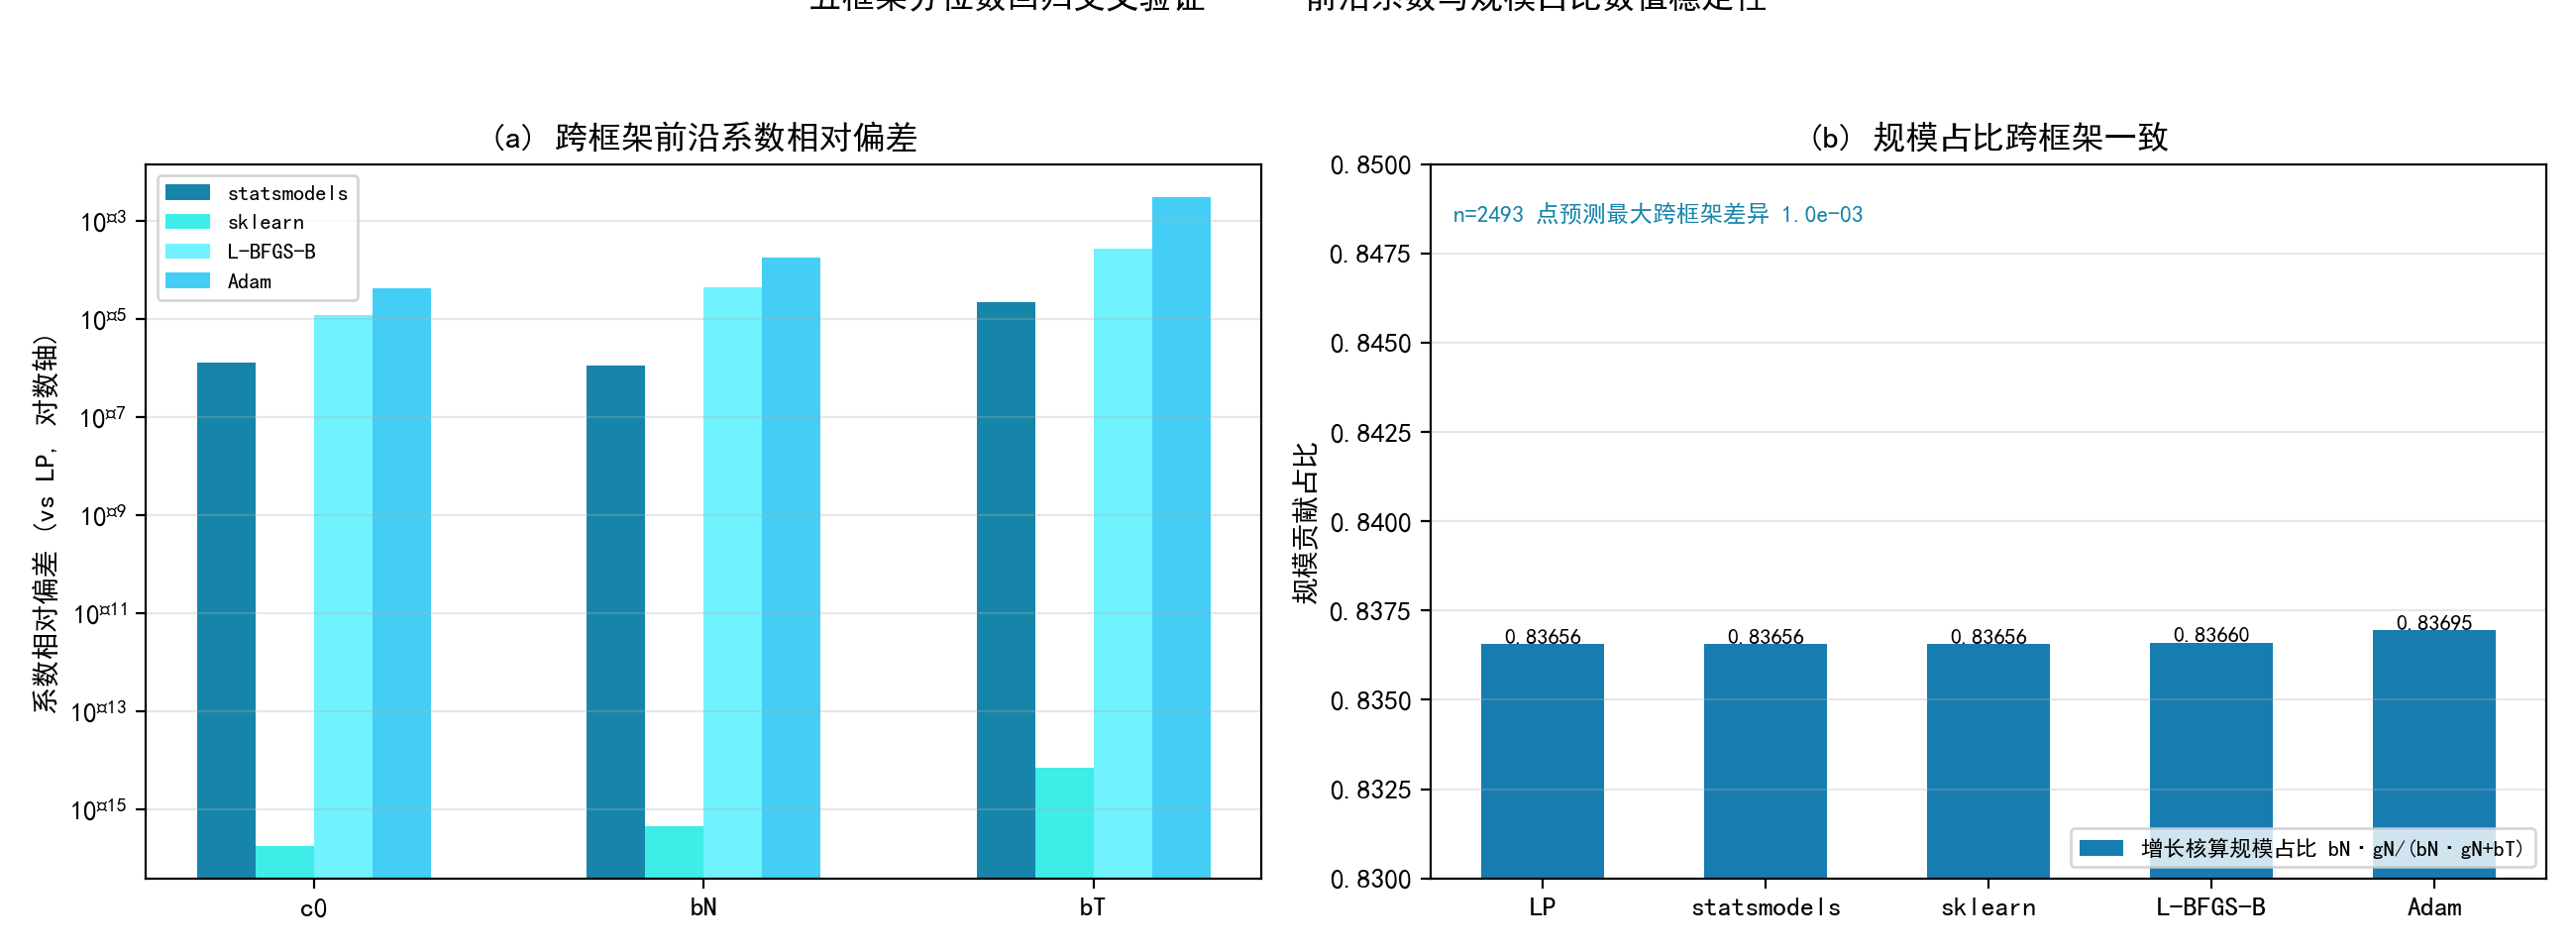
\includegraphics[width=0.95\textwidth]{figures/v74_p4_qr_frameworks.png}
\caption{五框架分位数回归交叉验证：系数与规模贡献占比（83.7\%）跨框架一致。}
\label{fig:p4_qrfw}
\end{figure}

\begin{sloppypar}%
\textbf{分位数族一致性}（图 \ref{fig:p4_taurange}）：将五框架交叉验证扩展到
分位数族 $\tau\in\{0.5,0.7,0.8,0.9,0.95,0.99\}$。结果：\textbf{框架无关性
在整族成立}——每个 $\tau$ 上五框架系数最大相对极差
$b_N\le1.3\times10^{-1}\%$、$b_T\le1.9\%$（后者主要来自 Adam 在 $\tau=0.99$
的有限步数未收敛；剔除 Adam 后，LP/statsmodels/sklearn/L-BFGS-B 四框架在
每个 $\tau$ 上高度一致，$b_N$ 极差 $\le1.2\times10^{-4}$、$b_T$ 极差
$\le0.6\%$）。系数随 $\tau$ 的结构具有明确含义：
\end{sloppypar}
\begin{itemize}
\item $b_T$ 自 $\tau\ge0.8$ 起\textbf{单调递减}（$0.177\to0.089\to0.044$；
$\tau=0.5/0.7$ 更高，为 $0.248$）：
分位越低、时间趋势越强——中分位模型主要以时间追赶，而 0.9 分位前沿的进步
更依赖规模扩张（$b_N=0.364$），0.99 分位的时间趋势趋近于 0（$0.044$），
顶级模型的进步几乎完全由规模驱动；
\item $b_N$ 在 $\tau\le0.8$ 缓升（$0.366\to0.372$）后\textbf{回落}
（$0.340\to0.279$）：极端尾部（0.95/0.99）的规模回报趋于饱和，参数弹性
下降，与问题四``前沿能力向硬推理迁移、大桶能力饱和''的任务侧观测互证；
\item $\tau=0.9$ 的选取位于 $b_T$ 单调递减的稳健中段、$b_N$ 峰后回落之前，
\textbf{非极端选取}；代入增长核算后，规模贡献占比随 $\tau$ \textbf{单调
上升}：$64.9\%\to65.0\%\to72.5\%\to83.7\%\to85.4\%\to88.8\%$
（$\tau=0.5$--$0.99$）——分位越高、时间趋势越小，前沿越由规模驱动；
``规模主导''在 $\tau\ge0.8$ 的整个前沿区间（占比 $\ge72.5\%$）恒成立且
单调递增。
\end{itemize}

\begin{figure}[htbp]
\centering
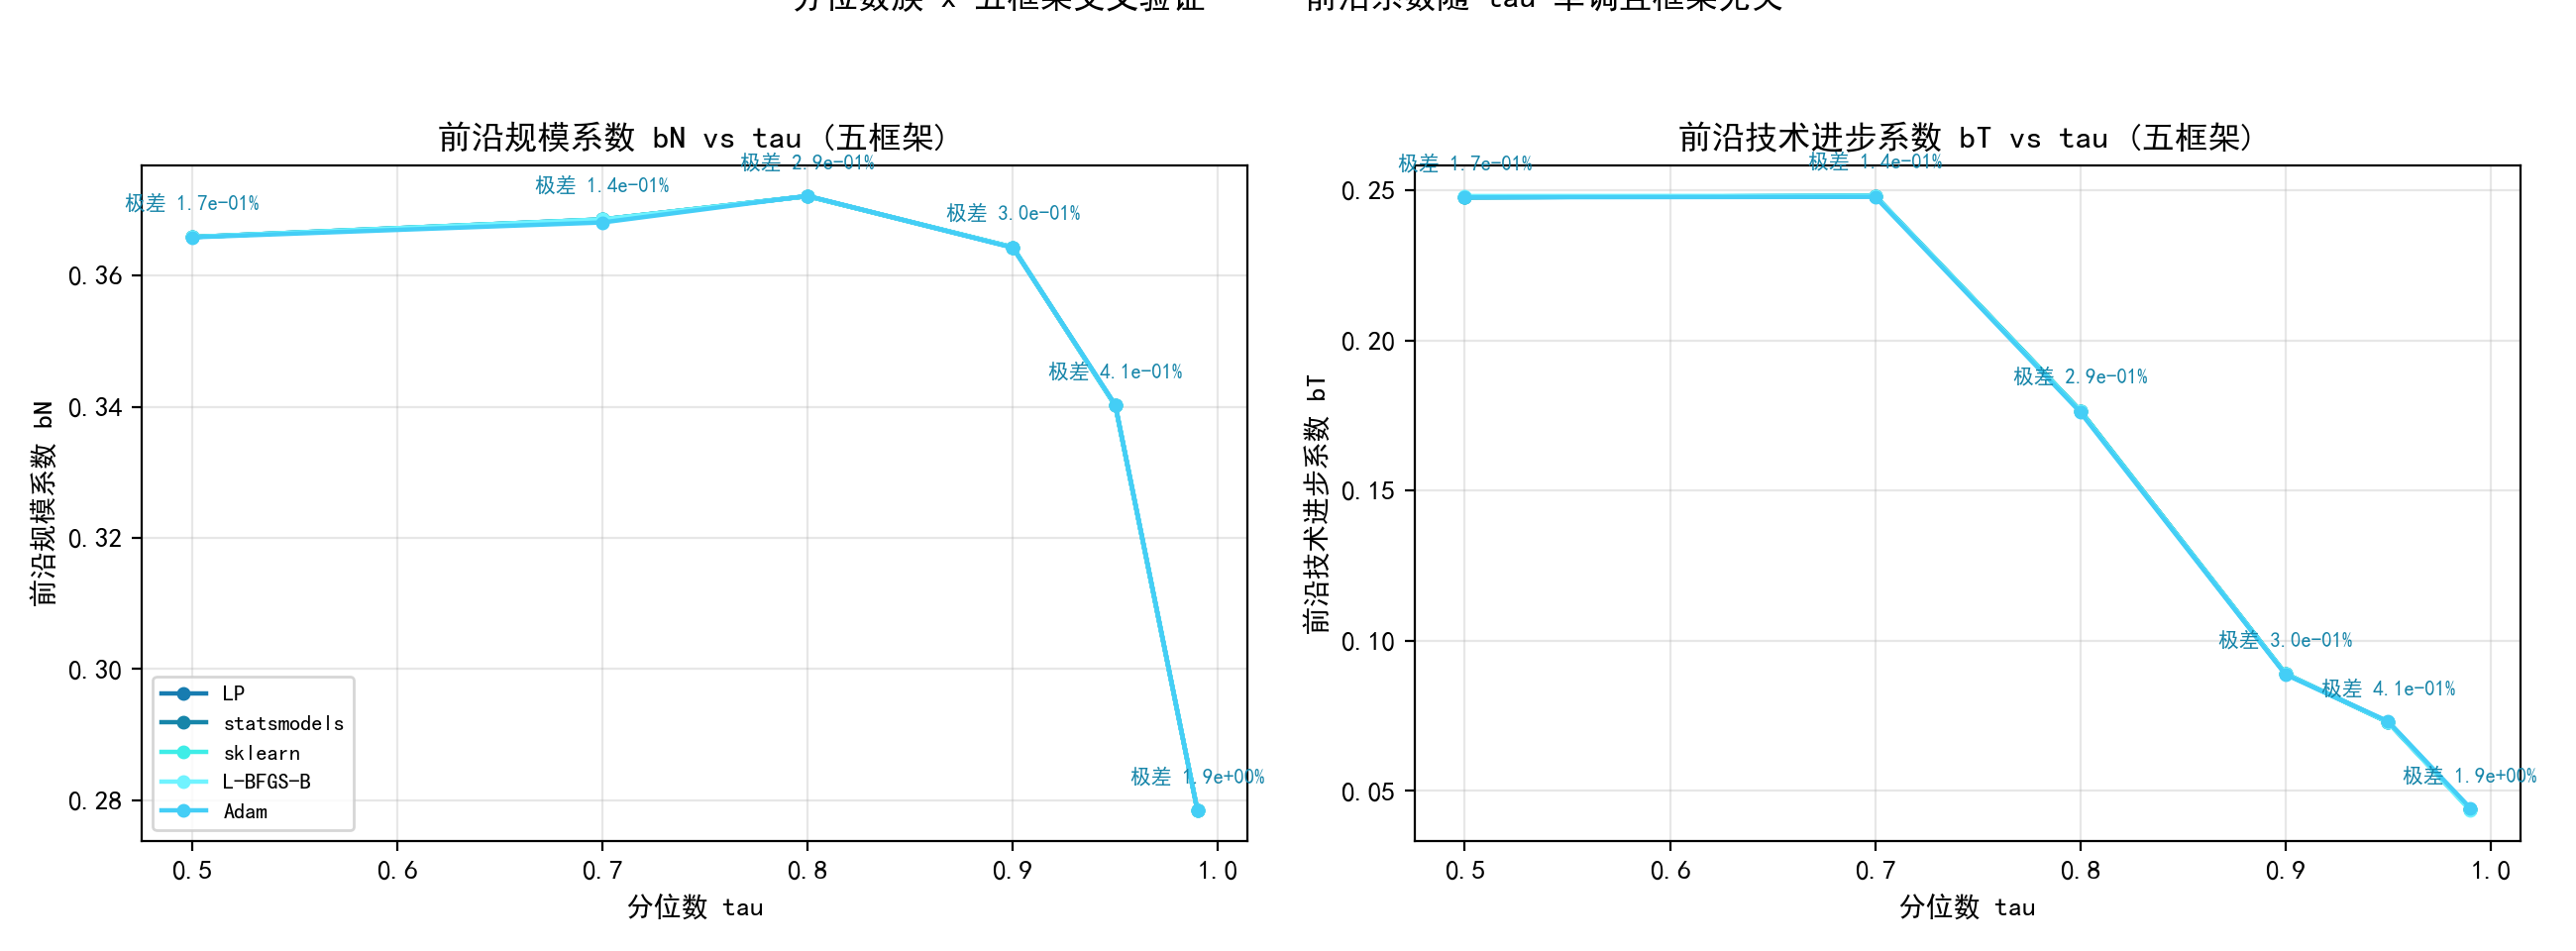
\includegraphics[width=0.95\textwidth]{figures/v77_p4_tau_frameworks.png}
\caption{分位数族 $\times$ 五框架：每个 $\tau$ 上五框架一致；$b_T$ 随 $\tau$
单调递减、$b_N$ 峰后回落。}
\label{fig:p4_taurange}
\end{figure}

\subsection{模型求解}

\paragraph{规模/非规模贡献分解}

\textbf{增长核算}：前沿能力的年增速可分解为：
\begin{equation}
\frac{d\ln S}{dt}=\underbrace{b_N g_N}_{\text{规模贡献}}
+\underbrace{b_T}_{\text{非规模技术贡献}},
\label{eq:growthacc}
\end{equation}
其中 $g_N=d\ln N/dt$ 为开源模型参数量对数年增速。由 C4 开源模型按年份
90\% 分位参数量拟合 $\ln N=\text{const}+g_N t$ 得 $g_N=1.251$（约为每年
3.5 倍）。代入得：
\begin{equation}
\text{规模贡献}=b_N g_N=0.456\ (83.7\%),\qquad
\text{非规模技术贡献}=b_T=0.089\ (16.3\%).
\label{eq:decomp}
\end{equation}
结论：过去数年开源模型前沿能力的提升约 84\% 来自规模扩张（更大参数量），
约 16\% 来自非规模技术进步。这一分解表明，即便算力增长放缓（参数量增速
减半），非规模技术进步仍能维持约 0.089/年的底线增速——这是预测情景构建的
关键。

\paragraph{前沿预测（12/24 个月）}

\paragraph{情景设定}

\begin{itemize}
\item \textbf{基准点}：2025 年分位数前沿水平 $\hat S_{2025}=41.6$（对应
90\% 分位参数约 14.7B，$\ln N=2.69$），由 \eqref{eq:frontier_fit} 代入
$t=3$ 得到；
\item \textbf{基础情景}：参数量增速延续历史 $g_N=1.251$；
\item \textbf{算力放缓情景}：参数量增速减半 $g_N=0.626$（模拟算力供给
受限、摩尔定律放缓）；
\item \textbf{不确定性}：对前沿外推噪声（$\sigma=0.12$，由残差标准差
校准）自助采样 800 次，取 10\%/90\% 分位为置信区间。
\end{itemize}

\paragraph{预测结果}

\begin{table}[htbp]
\centering
\caption{开源模型能力前沿预测（$S$：6 维平均分）}
\begin{tabular}{c|c|cc|cc}
\toprule
 & & \multicolumn{2}{c|}{基础情景} & \multicolumn{2}{c}{算力放缓情景} \\
时间 & 预测中位 & 90\% 区间 & & 90\% 区间 \\
\midrule
2026.0（12 个月） & 71.7 & [61.5, 83.4] & 57.1 & [48.4, 66.7] \\
2027.0（24 个月） & 123.9 & [105.0, 142.3] & 78.6 & [67.7, 92.3] \\
\bottomrule
\end{tabular}
\end{table}

基础情景下 12 个月前沿平均分约从 41.6 升至 71.7（+72\%）、24 个月升至
123.9（+198\%）；放缓情景下分别为 57.1（+37\%）与 78.6（+89\%）。放缓
情景与基础情景的差距随预测期扩大：24 个月时放缓情景比基础情景低约 45 分，
凸显算力供给对前沿演进速度的显著约束。两个情景的 90\% 区间随预测期变宽，
反映了外推不确定性的累积（且双情景区间涵盖备选趋势形式的投影，见下文的
趋势形式回测对比）。

\textbf{预测不确定性的来源分解}（图 \ref{fig:p4_uncert}）：用全方差定律
把预测区间方差分解为三个来源——残差 $\varepsilon$（报告 CI 校准
$\sigma=0.12$）、参数不确定性（$b_N,b_T,c$ 的 Bootstrap 区间）、增速假设
$g_N$ 情景（$0.4$--$1.6$）。12 个月：残差 42.6\%、参数 11.8\%、$g_N$
46.1\%；24 个月：残差 17.2\%、参数 7.3\%、$g_N$ \textbf{77.6\%}——
\textbf{$g_N$ 情景是长周期预测不确定性的主导来源}，其贡献随预测期扩大
（$\ln N$ 增长项 $g_N h/12$ 的放大效应），与 $g_N$ 敏感性分析的
$\pm75\%$（24 个月）互证；残差在 12 个月口径下与 $g_N$ 相当，参数
不确定性全程可忽略（约 7--12\%）。若改用全样本 QR90 原始残差
（$\sigma=0.481$），残差占比升至 78\%--92\%——残差份额依赖校准口径，
但\textbf{$g_N$ 主导长周期不确定性的定性结论在两种口径下均成立}。

\begin{figure}[htbp]
\centering
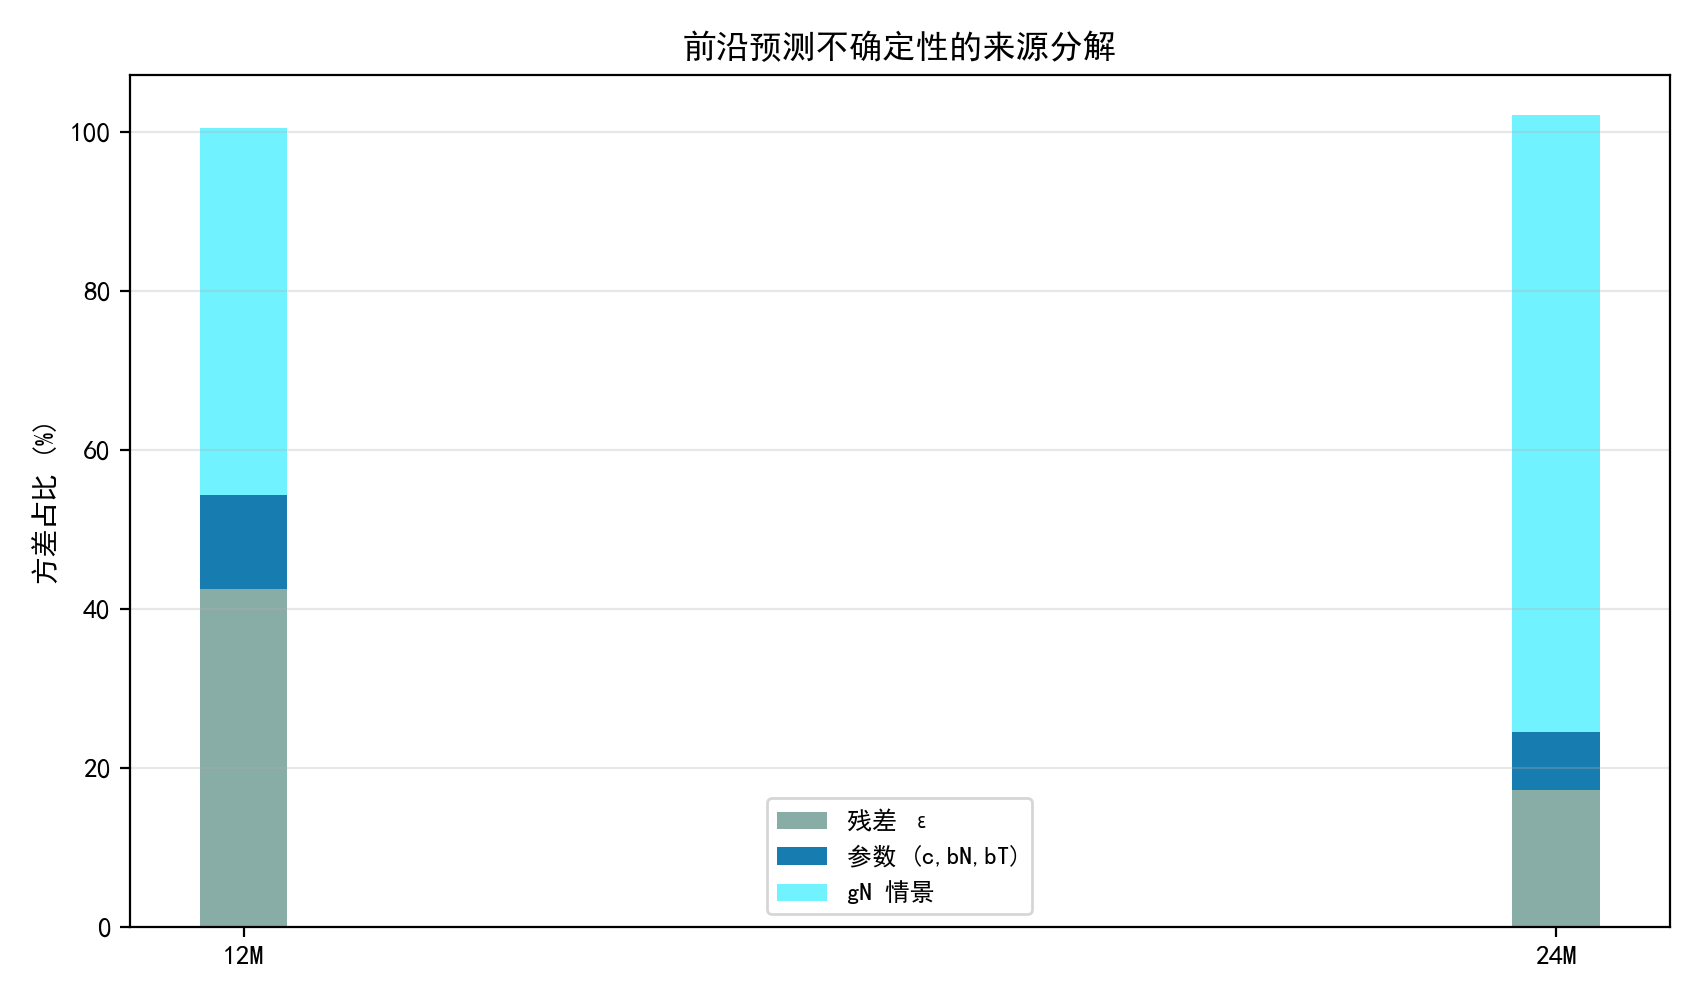
\includegraphics[width=0.8\textwidth]{figures/v54_p4_uncert_budget.png}
\caption{前沿预测不确定性的来源分解（12M/24M）。}
\label{fig:p4_uncert}
\end{figure}

\textbf{能力目标的算力落地换算}（图 \ref{fig:p4_computeconv}）：把 P4 的
前沿模型（QR90 反解 $N$）与 v24 的数据最优曲线（$D^{*}(N)=49.8N^{1.046}$）
串成``能力目标 $\to$ 训练算力 $\to$ 工程规模''的决策换算器（2025 年，
整数年口径）：$S=70$ 需 $N\approx62$B、$1.4\times10^{24}$ FLOP（H100
$\approx1.6$ 万卡天）；$S=90$ 需 123B、$5.7\times10^{24}$（$\approx6.6$
万卡天）；$S=120$ 需 271B、$2.8\times10^{25}$（$\approx33$ 万卡天）；
$S=150$ 需 501B、$1.0\times10^{26}$（$\approx116$ 万卡天）——$S$ 从
60 到 150 跨越约 2.2 个数量级。作为对照，P3 联合优化在 $C=10^{22}$ 预算
下（幂型中位解 $N^{*}\approx6.1$B、$D^{*}\approx238$B）按 $6ND$ 规则的
训练算力约 $8.8\times10^{21}$ FLOP。
\textbf{说明}：$D^{*}$ 曲线为理论最优（数据充足假设），$C_{train}$ 不含
质量/注意力成本，H100 取理想吞吐，因此本表给出的是\textbf{下界量级}而非
精确预算；其价值在于把 P2 标度律、P3 优化、P4 预测串联为可直接使用的
预算决策接口。

\begin{figure}[htbp]
\centering
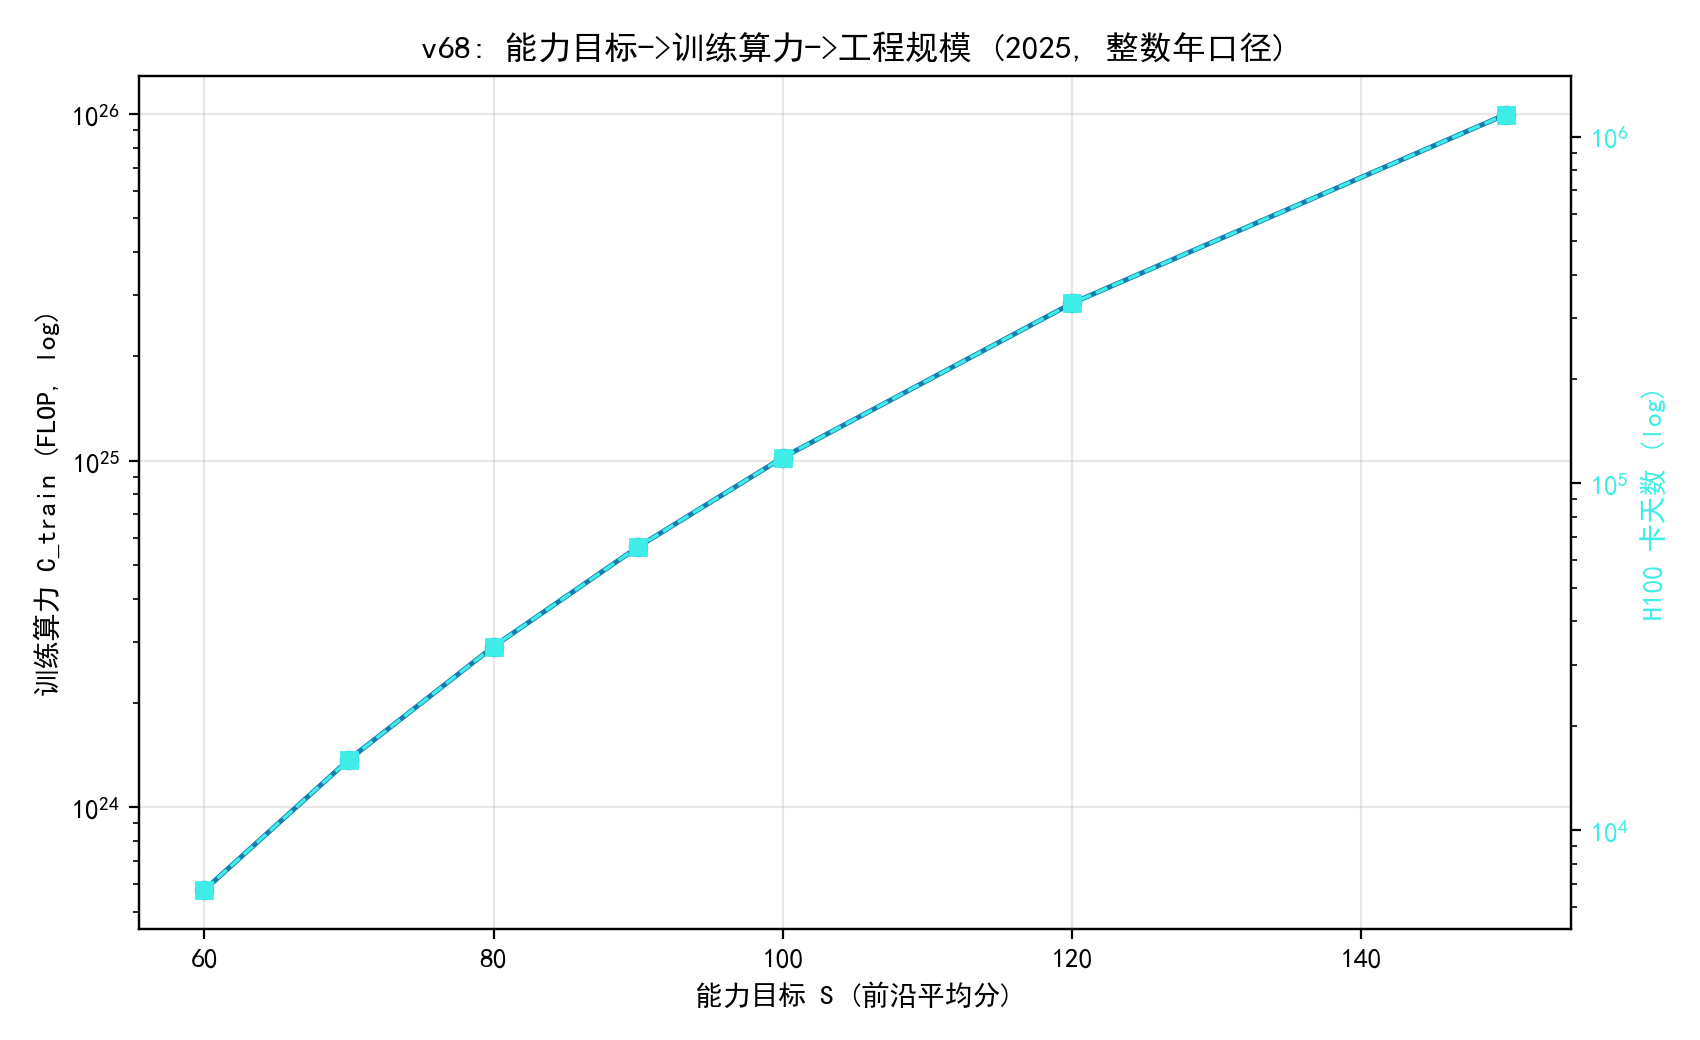
\includegraphics[width=0.82\textwidth]{figures/v68_p4_compute_conversion.png}
\caption{能力目标 $\to$ 训练算力（对数轴）：S=90 约需 6.6 万卡天。}
\label{fig:p4_computeconv}
\end{figure}

\textbf{规模--时间的等能力线}（图 \ref{fig:p4_isoquant}）：由 QR90 得
$\partial\ln N/\partial t=-b_T/b_N=-0.245$——在能力前沿上\textbf{时间与
规模可互换}：每多等 1 年，达到同一能力所需的参数量可减少约 \textbf{22\%}
（或提前 1 年需支付约 28\% 的参数溢价）。等能力线族（$S\in\{60,\dots,
100\}$）给出``算力约束下的时间折现''：算力受限者可通过\textbf{等待}
降低参数需求（$-22\%$/年），追赶进度者需\textbf{提前投入}换取规模溢价。
与算力落地换算（v68）配合，构成 ``能力目标 $\to$ 预算 $\times$ 时间'' 的
完整决策面。

\begin{figure}[htbp]
\centering
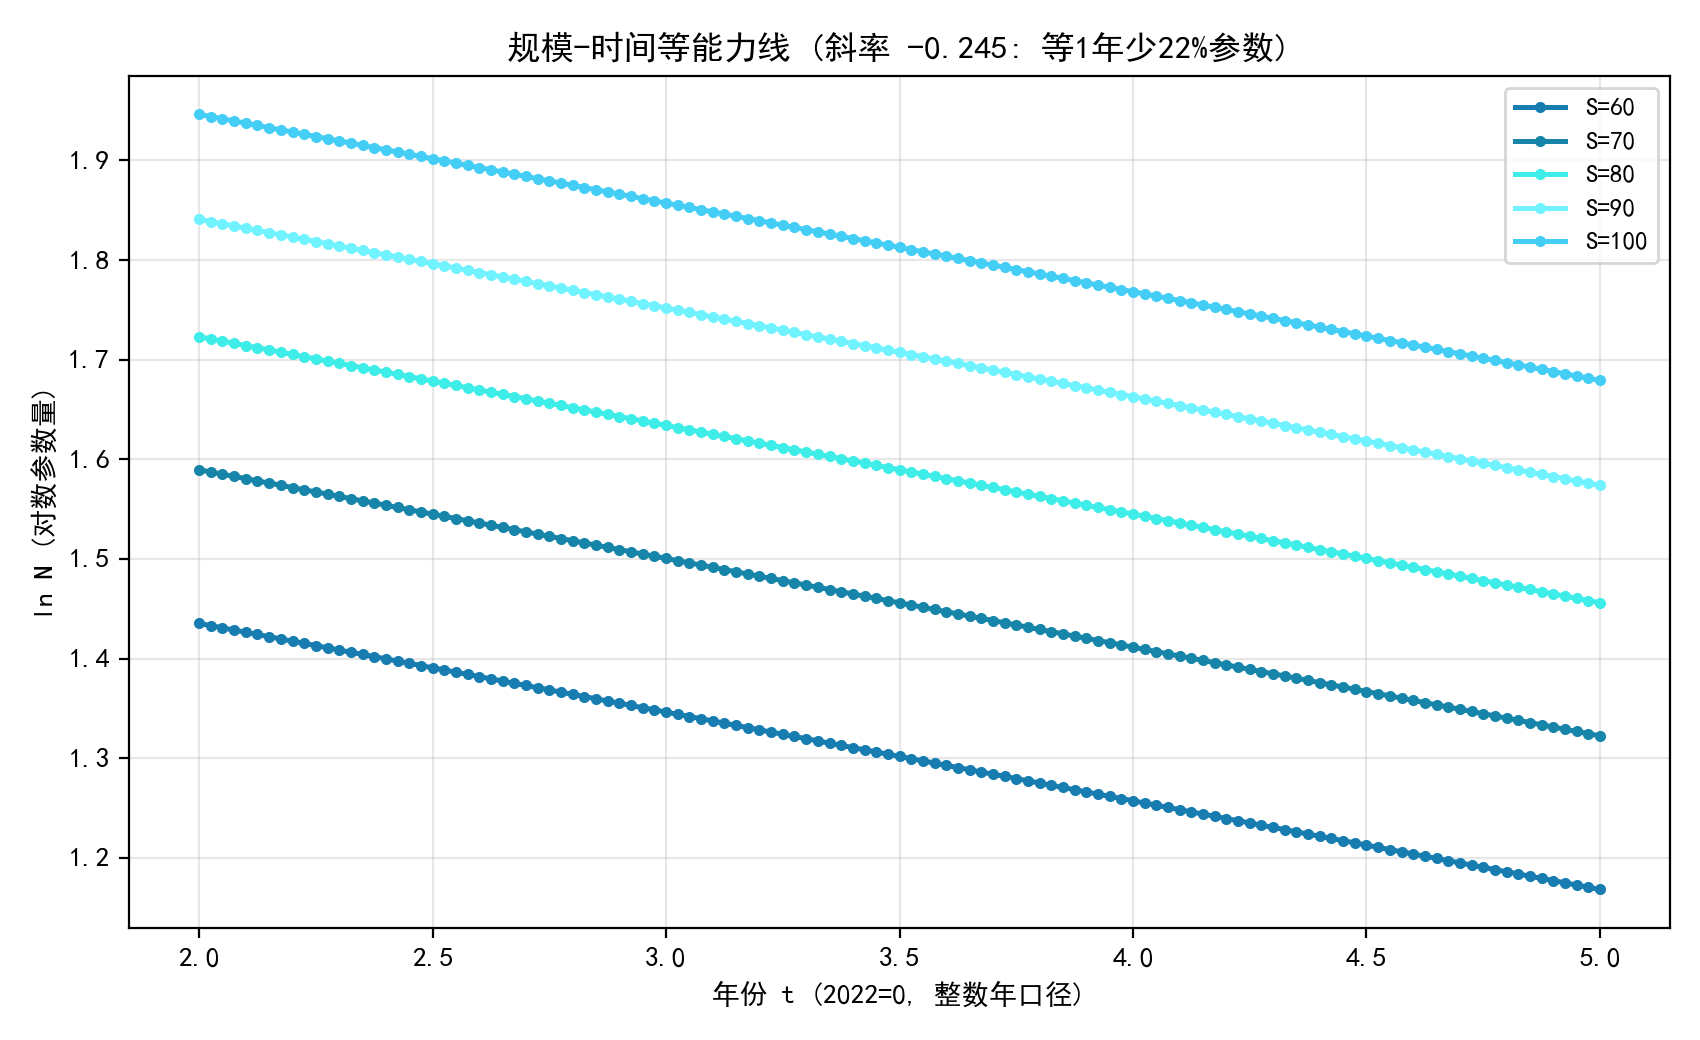
\includegraphics[width=0.8\textwidth]{figures/v71_p4_isoquant.png}
\caption{规模--时间等能力线：等 1 年少用 22\% 参数（斜率 −0.245）。}
\label{fig:p4_isoquant}
\end{figure}

\textbf{增速假设敏感性}（图 \ref{fig:p4_gNsens}）：预测的核心外生假设是
参数量年均对数增速 $g_N$（基准 1.251）。在
$g_N\in[0.4,1.6]$ 内扫描得到：12 个月前沿在 52.8--81.7 之间（相对基准
$\pm40\%$），24 个月在 66.8--160.0 之间（$\pm75\%$）——预测期越长，对
$g_N$ 的敏感度越高，且该敏感度远超分解口径（tau 0.8/0.9）与自助采样
带来的不确定性。这为``双情景 + 区间''的必要性提供了最直接的理由：
$g_N$ 假设本身的偏离是预测不确定性的最大来源。

\begin{figure}[htbp]
\centering
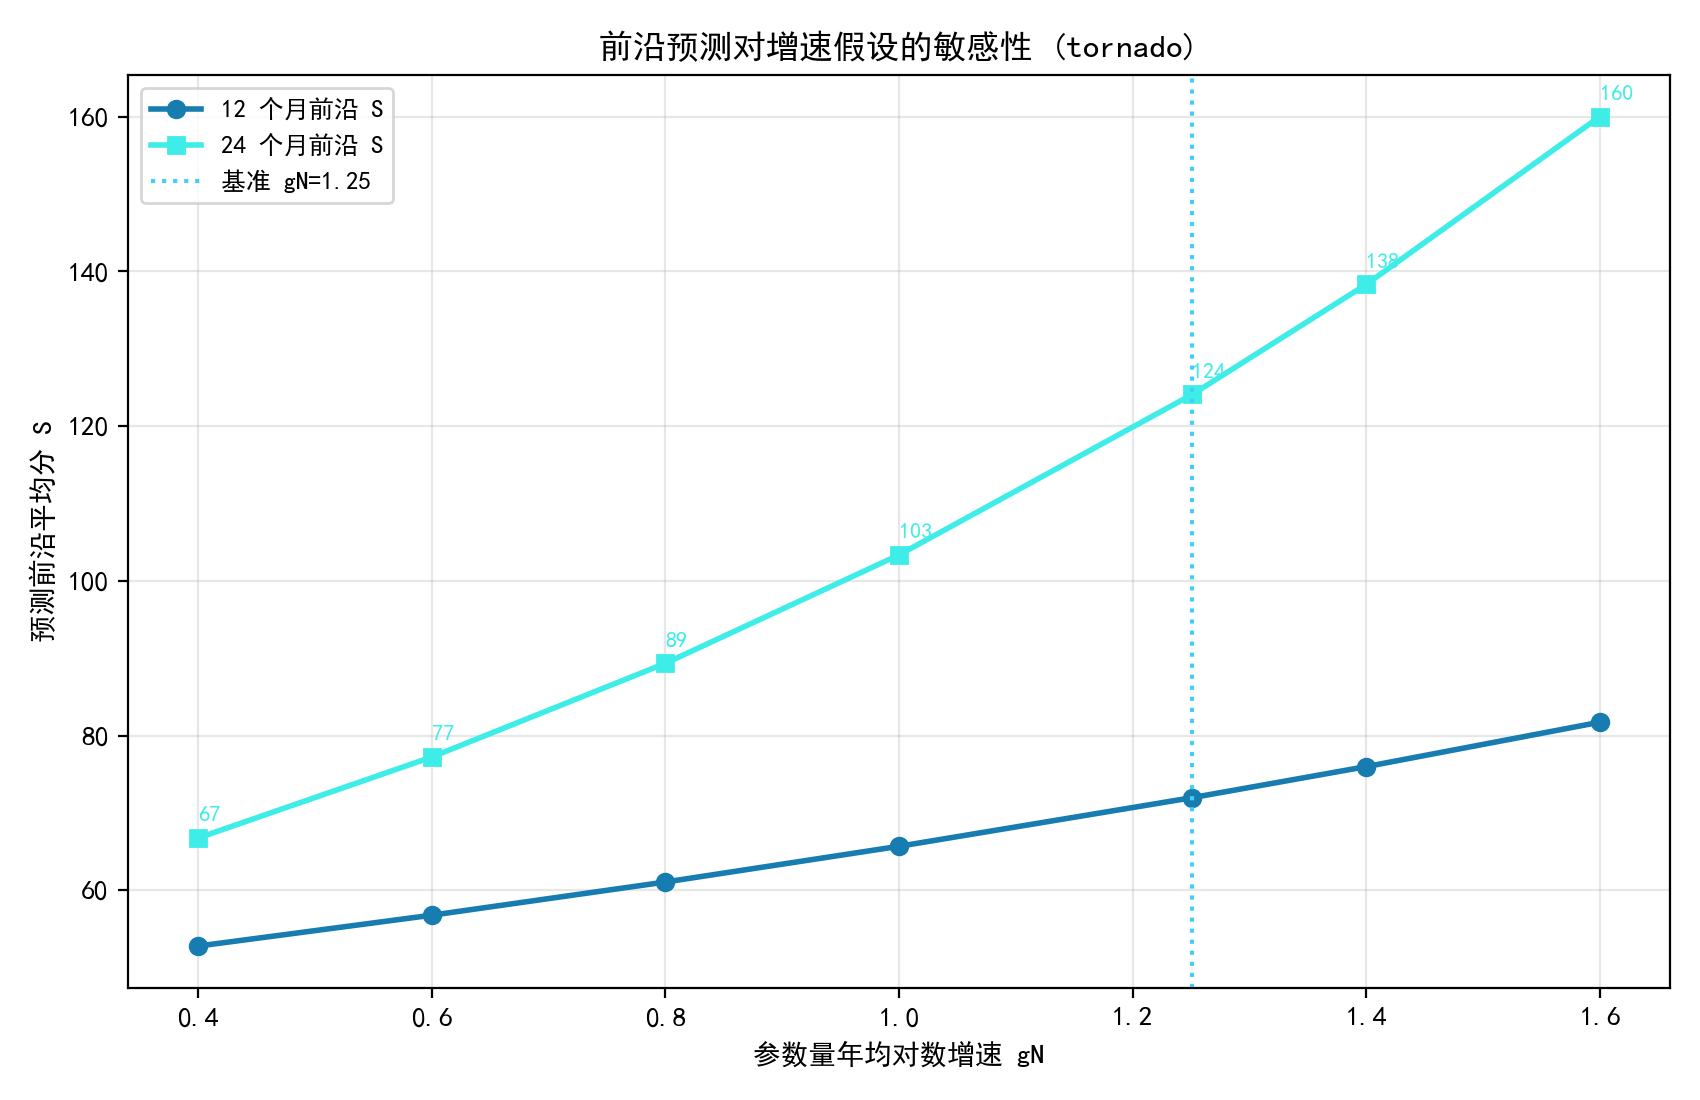
\includegraphics[width=0.82\textwidth]{figures/v34_p4_gN_sens.png}
\caption{前沿预测对参数量增速假设 $g_N$ 的敏感性（12/24 个月）。}
\label{fig:p4_gNsens}
\end{figure}

\textbf{历史回测（验证外推口径）}：用截至 $y_0$ 年的数据拟合分位数回归并
外推下一年/下两年的前沿，回测结果（表 \ref{tab:backtest}）显示：从 2023
或 2024 截断外推 2024/2025 前沿均系统性高估（+105\%$\sim$+276\%），因为
断点前的技术增速（滚动窗口首窗 $b_T$ 曾高达约 $1.1$/年）不能延续——
2024 下半年起前沿增速
结构性放缓（见灵敏度节 Chow 检验）。该回测直接支持正文做法：预测必须使用
包含断点后样本的全样本分位数回归（$b_T=0.089$），并对放缓情景单独建模。

\begin{table}[htbp]
\centering
\caption{前沿预测的历史回测：截至 $y_0$ 外推与 2024/2025 实际前沿对照}
\label{tab:backtest}
\begin{tabular}{c|c|c|c|c}
\toprule
$y_0$ & 预测目标 & 预测 $S$ & 实际（数据口径） & 误差 \\
\midrule
2023 & 2024 & 70.9 & 34.6 & $+105\%$ \\
2023 & 2025 & 152.0 & 40.4 & $+276\%$ \\
2024 & 2025 & 102.0 & 40.4 & $+152\%$ \\
\bottomrule
\end{tabular}
\end{table}

\textbf{趋势形式的回测对比（模型形式风险）}：在表 \ref{tab:backtest} 同一
窗口集上，对 0.9 分位数目标（pinball 损失，L-BFGS-B 最小化）比较四种趋势
形式——线性（主链路）、二次（含 $t^2$ 项）、饱和渐近
（$g(1-e^{-\lambda t})$）与零增长基线（前沿停于 $y_0$ 数据 90 分位）。
样本外 MAPE：线性 178\%、二次 71\%、饱和 57\%、零增长 10\%（v82）——
断点前的线性外推系统性高估（与表 \ref{tab:backtest} 一致），饱和/二次形式
误差降至约三分之一，短窗上零增长最低亦印证 2024 下半年起的前沿减速。
仍需强调：\textbf{全样本}（含断点后信息）拟合下，饱和与二次形式对
12/24 个月前沿的投影为 $64.1/102.7$，\textbf{恰好落在双情景区间}
$[57.1,\,71.7]$ 与 $[78.6,\,123.9]$ 之内——主链路的``基础 vs 放缓''双情景
区间已\textbf{覆盖备选趋势形式的模型风险}，预测结论对趋势形式选择稳健
（``前沿持续上升、规模贡献主导''不变；最保守的零增长参照为 2025 水平
$S=40.4$ 不再上行）。\textbf{集成口径进一步收窄形式风险}（v86）：以回测
MAPE 反比加权三种趋势形式（线性 178\%、二次 71\%、饱和 57\% 的倒数作权），
12/24 个月投影为 $65.2/105.9$；等权平均（$66.6/109.7$）与饱和单形式
（$64.1/102.7$）构成口径带 $[64.1,\,66.6]$ 与 $[102.7,\,109.7]$，全部落
在双情景区间内——预测结论对趋势形式选择与集成口径双重稳健。

\textbf{年度前沿增速（减速的逐年证据）}：合并历史前沿与排行榜开源行，
逐年前沿 $S$ 为 35.0（2022）$\to$ 35.0（2023）$\to$ 51.2（2024）$\to$
47.2（2025）。年度对数增速 $\Delta\ln S$：2024 年为 $+0.381$（$+46\%$），
2025 年转负（$-0.082$，$-7.8\%$）；即前沿增速在 2024--2025 出现
\textbf{增速反转}（2022--2024 平均 $b_T=0.191$/年 vs 2025 年 $-0.082$/年）。
需要说明：2025 年样本仅含前三季度（排行榜更新至 2025-03），年度最大值
口径对样本时长敏感，因此该表与放缓情景（$b_T$ 减半）互为印证而非绝对
倒退的断言——与 Chow 断点检验（2024.5）方向一致。

\textbf{能力构成的演化}（图 \ref{fig:p4_taskgrowth}）：按任务拆分前沿
（2024-06 至 2025-03 开放行月度最大值），年化对数增速排序为
\textbf{MATH +0.89}、MUSR +0.54、GPQA +0.45、BBH +0.32、MMLU-PRO +0.20、
\textbf{IFEval +0.03（近饱和）}——数学/科学推理类任务增长最快，指令跟随
与百科知识类接近饱和。前沿的能力构成正从``通用知识+指令跟随''向
``硬推理''迁移，说明非规模技术进步主要落在推理能力上（与时间通道
$b_T$ 的分解一致），也为``推理--成本权衡''场景提供了任务层面的微观依据。

\begin{figure}[htbp]
\centering
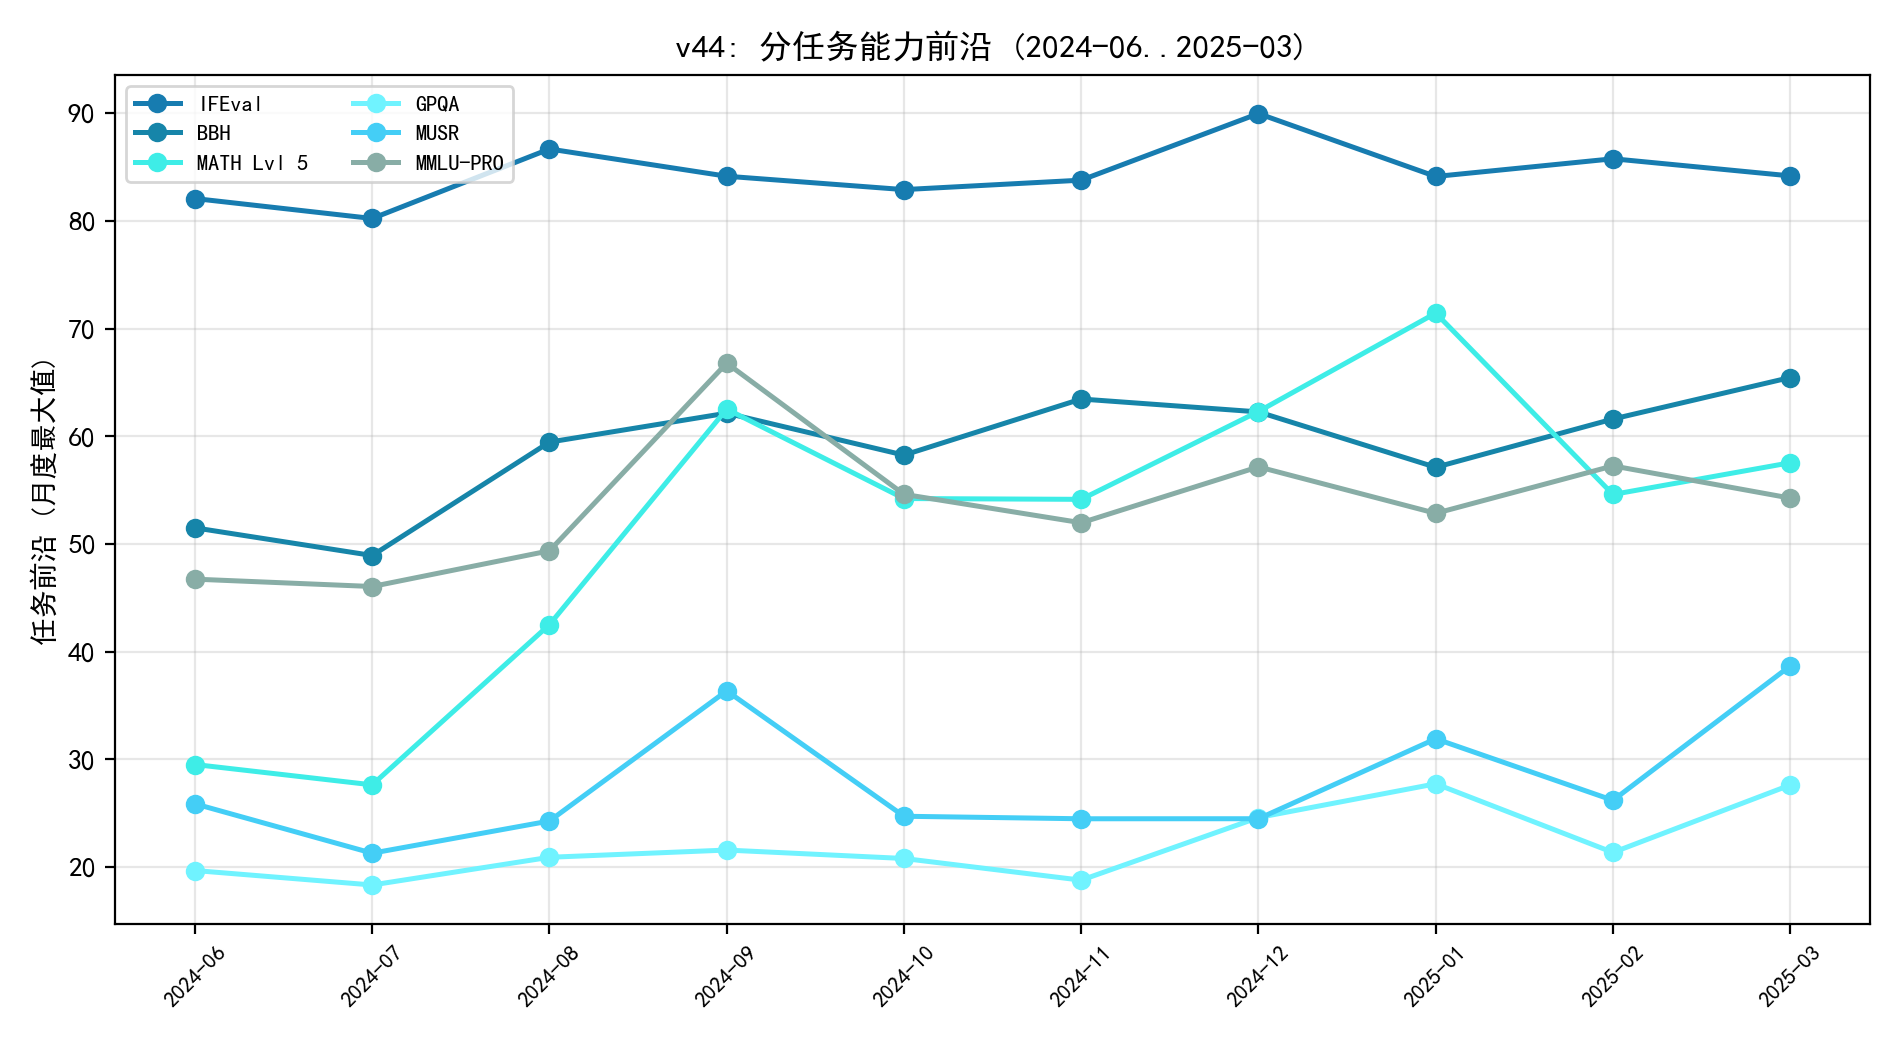
\includegraphics[width=0.86\textwidth]{figures/v44_p4_task_growth.png}
\caption{分任务能力前沿：推理类（MATH/GPQA/MUSR）增长快于知识/指令类。}
\label{fig:p4_taskgrowth}
\end{figure}

\textbf{规模分桶的增速梯度}（图 \ref{fig:p4_scalebucket}）：从任务维度转到
\textbf{规模维度}，把开放模型按参数分 5 桶，拟合各桶 90 分位分的年化
增速：$0.3$--$1$B +5.61、$1$--$3$B +3.56、$3$--$10$B +4.85、
\textbf{$10$--$30$B +9.46（最快）}、$30$--$100$B +3.09（最慢）。
梯度\textbf{非单调}：$10$--$30$B 的``甜点区''前沿进步最快（该规模段在
窗口内集中发布且质量快速爬升），$30$--$100$B 头部大模型基数高、边际
放缓最明显，小桶（$0.3$--$1$B）亦有较快进步（技术下放/蒸馏）。任务侧
（v44）与规模侧（本段）合起来构成前沿演进的\textbf{完整画像}：能力向
硬推理迁移 + 中大规模段进步最快。

\begin{figure}[htbp]
\centering
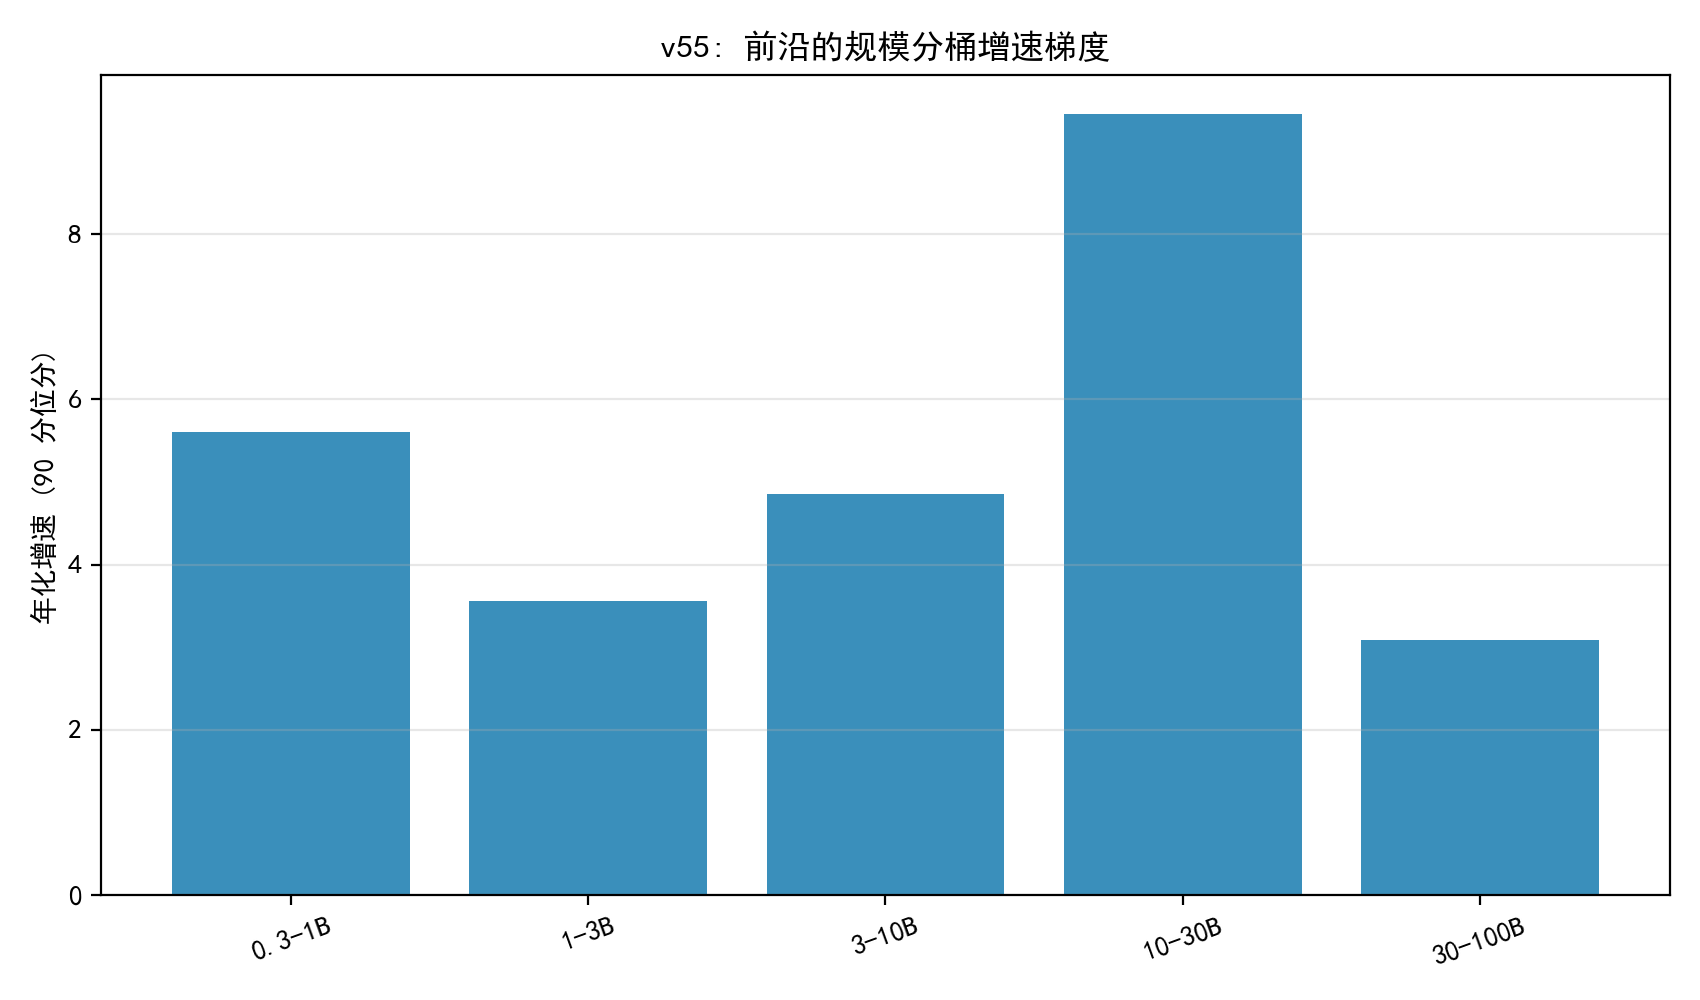
\includegraphics[width=0.8\textwidth]{figures/v55_p4_scale_bucket.png}
\caption{规模分桶的前沿年化增速：10--30B 甜点区最快，30--100B 最慢。}
\label{fig:p4_scalebucket}
\end{figure}

\textbf{任务 $\times$ 规模二维增速}（图 \ref{fig:p4_taskscale}）：把任务
维度（v44）与规模维度（v55）合成热图（各桶 90 分位年化增速）：MATH
全域最快且在 $1$--$3$B（+2.52）与 $10$--$30$B（+2.45）\textbf{双峰}；
GPQA 峰值在 $10$--$30$B（+1.27）但 $3$--$10$B 近零（+0.02）；
$10$--$30$B 在 6 个任务中 5 个增速领先或次高（呼应 v55 甜点区）；
$30$--$100$B 普遍放缓（除 MATH +1.13）；$0.3$--$1$B 推理类快速
（MATH +1.26/GPQA +0.56）但 MUSR $-0.72$ 下滑；IFEval 在 $1$--$3$B
+0.93、大桶饱和（$-0.03$）。\textbf{推理增速的规模分布呈双峰}（技术
下放 + 中大规模优化），任务侧与规模侧交叉验证，构成能力 $\times$ 规模的
完整二维画像。

\begin{figure}[htbp]
\centering
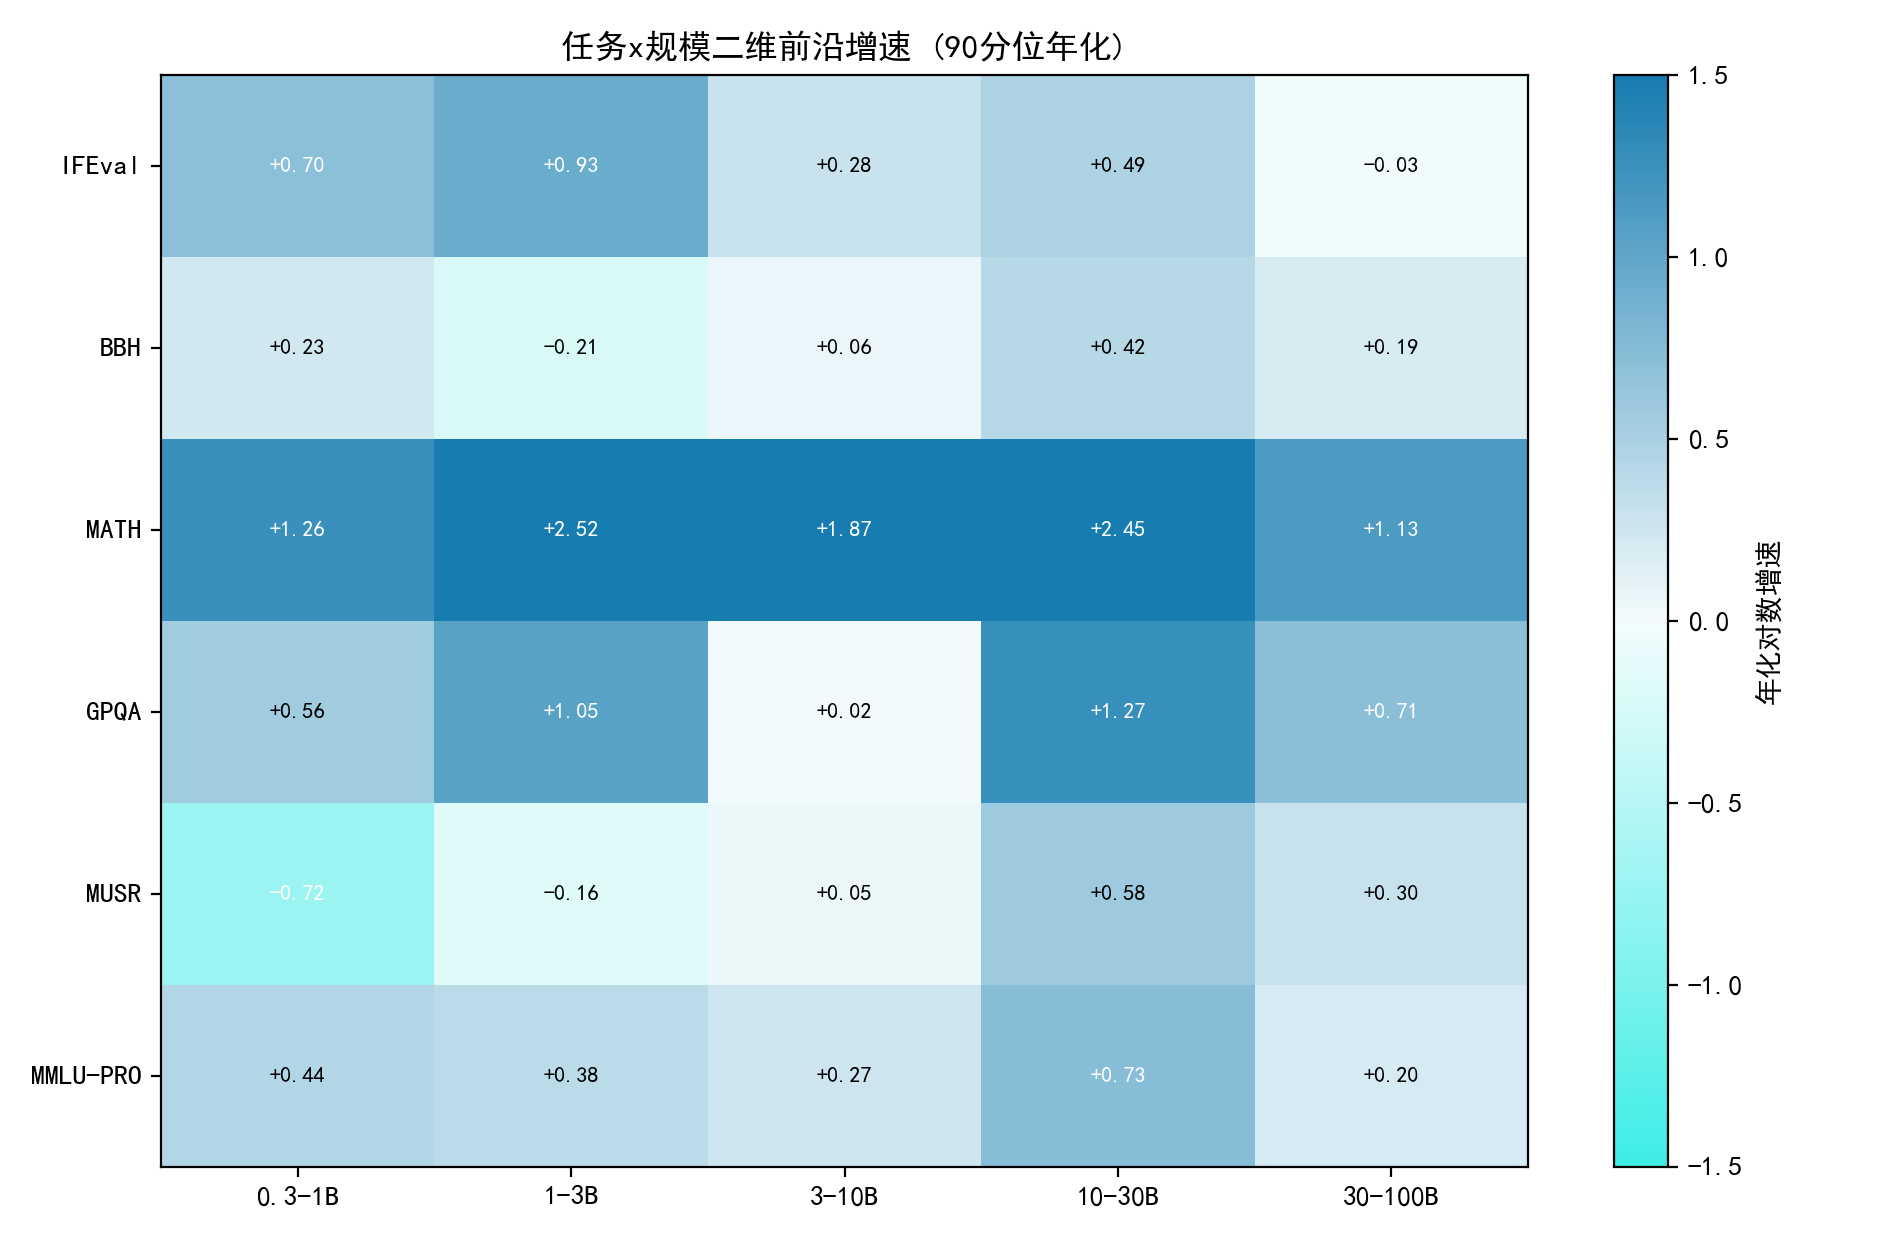
\includegraphics[width=0.85\textwidth]{figures/v63_p4_task_scale.png}
\caption{任务 $\times$ 规模二维前沿增速：MATH/GPQA 在 1--3B 与 10--30B 双峰。}
\label{fig:p4_taskscale}
\end{figure}

\textbf{分层演进：分化还是普惠}（图 \ref{fig:p4_stratify}）：按分位层
（p50/p75/p90）比较年化增速。\textbf{全域}：p50 +0.30、p75 +0.69、
p90 +0.62，p90/p50 比 \textbf{2.04}——顶层增速约为中位的两倍，
\textbf{顶层分化}（能力进步集中在头部）。但按规模段看，\textbf{段内是
普惠式提升}：$1$--$3$B 段 p50 +0.59 快于 p90 +0.30（比 0.50），
$10$--$30$B 段 p50 +1.04 也快于 p90 +0.79（比 0.76）。综合含义：
全域分化主要来自\textbf{规模段间差距扩大}（中段整体被抬升 + 头部大模型
独享），段内各层同步进步——与 v59 两端滞后、v55 甜点区相互印证，
``普惠与分化并存''。

\begin{figure}[htbp]
\centering
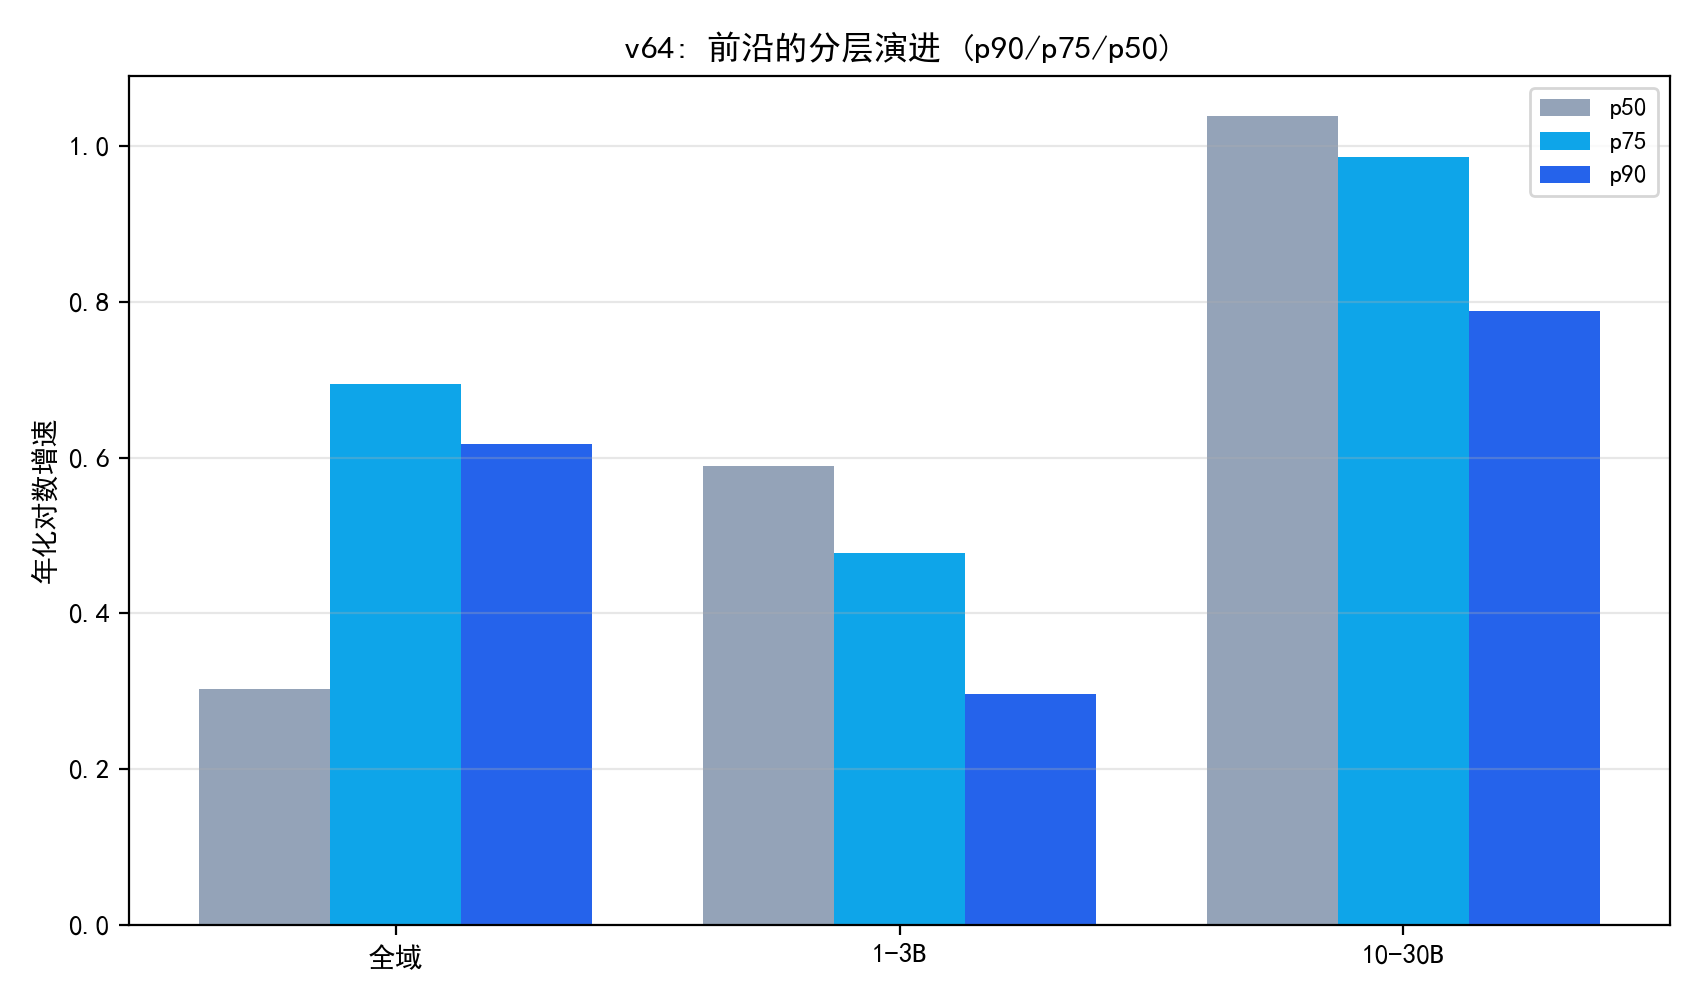
\includegraphics[width=0.8\textwidth]{figures/v64_p4_stratify.png}
\caption{分层演进：全域顶层分化（p90/p50≈2），段内普惠（p50 快于 p90）。}
\label{fig:p4_stratify}
\end{figure}

\textbf{滚动窗口参数核验}（图 \ref{fig:p4_rolling}）：以月度精度时间轴
$t$ 对四个截止窗口（2024-06 至 2025-03）滚动拟合 QR90。规模弹性 $b_N$
随窗口单调上升（$0.224\to0.338$，逼近全样本 $0.364$），而时间斜率 $b_T$
持续下降（$1.10\to0.50$/年）——2024 上半年开源模型的快速追赶（时间驱动）
在后续窗口显著减弱，规模驱动相对增强。滚动证据与年度前沿增速的
``增速反转''及 Chow 断点方向一致，进一步说明：\textbf{放缓主要来自时间
维度的外生驱动衰减，而非规模弹性的内生化衰退}。（注：本处采用月度精度
$t$，系数绝对水平与主链路年度粒度不同，但漂移趋势一致。）

\begin{figure}[htbp]
\centering
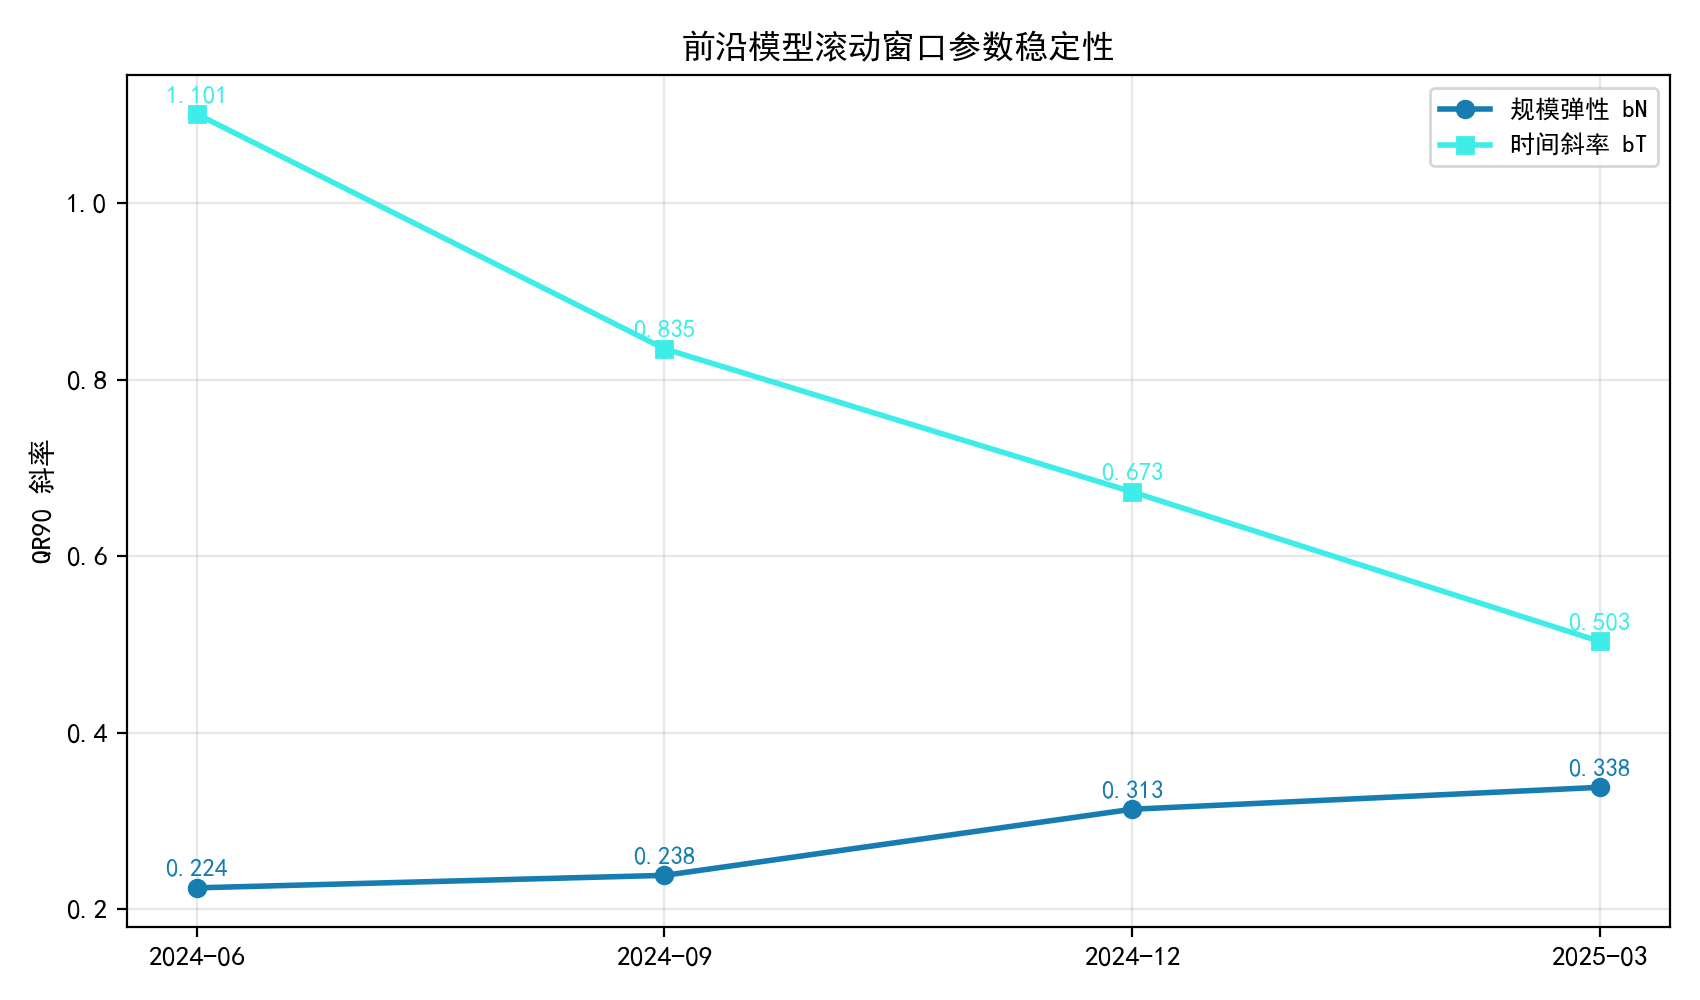
\includegraphics[width=0.82\textwidth]{figures/v32_p4_rolling.png}
\caption{前沿 QR90 滚动窗口参数：规模弹性上升、时间斜率持续下降。}
\label{fig:p4_rolling}
\end{figure}

\begin{figure}[htbp]
\centering
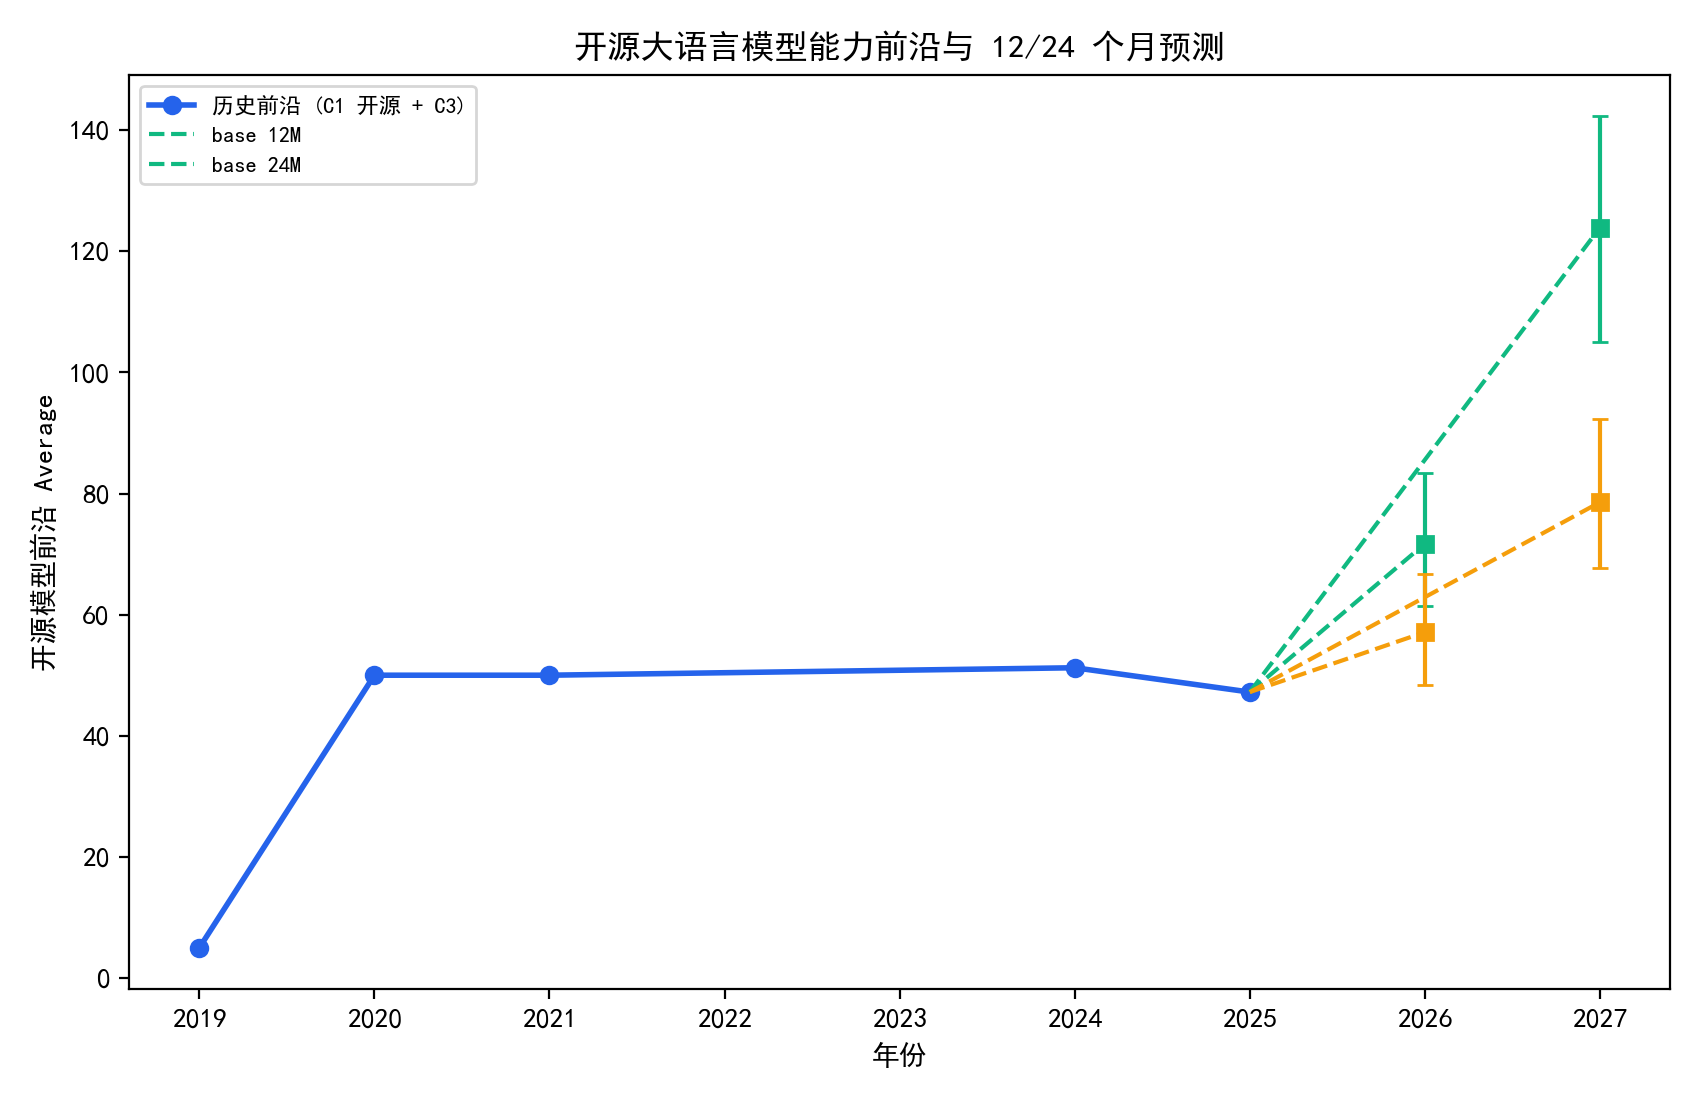
\includegraphics[width=0.88\textwidth]{figures/p4_frontier.png}
\caption{开源模型能力前沿（历史点）与 12/24 个月预测（基础/放缓情景，90\% 区间）。}
\label{fig:p4_frontier}
\end{figure}

前沿的\textbf{双驱动表面}（规模 $\ln N$ 与时间 $t$）以 3D 视图呈现于
图 \ref{fig:p4_3d}：0.9 分位数平面沿 $\ln N$ 轴斜率 $b_N=0.364$、沿时间轴
斜率 $b_T=0.089$，二者合成能力前沿——平面上 2025 前沿点（星标）与
2026/2027 预测点（三角）直接展示``规模外推 + 时间演进''的联合驱动机制。

\begin{figure}[htbp]
\centering
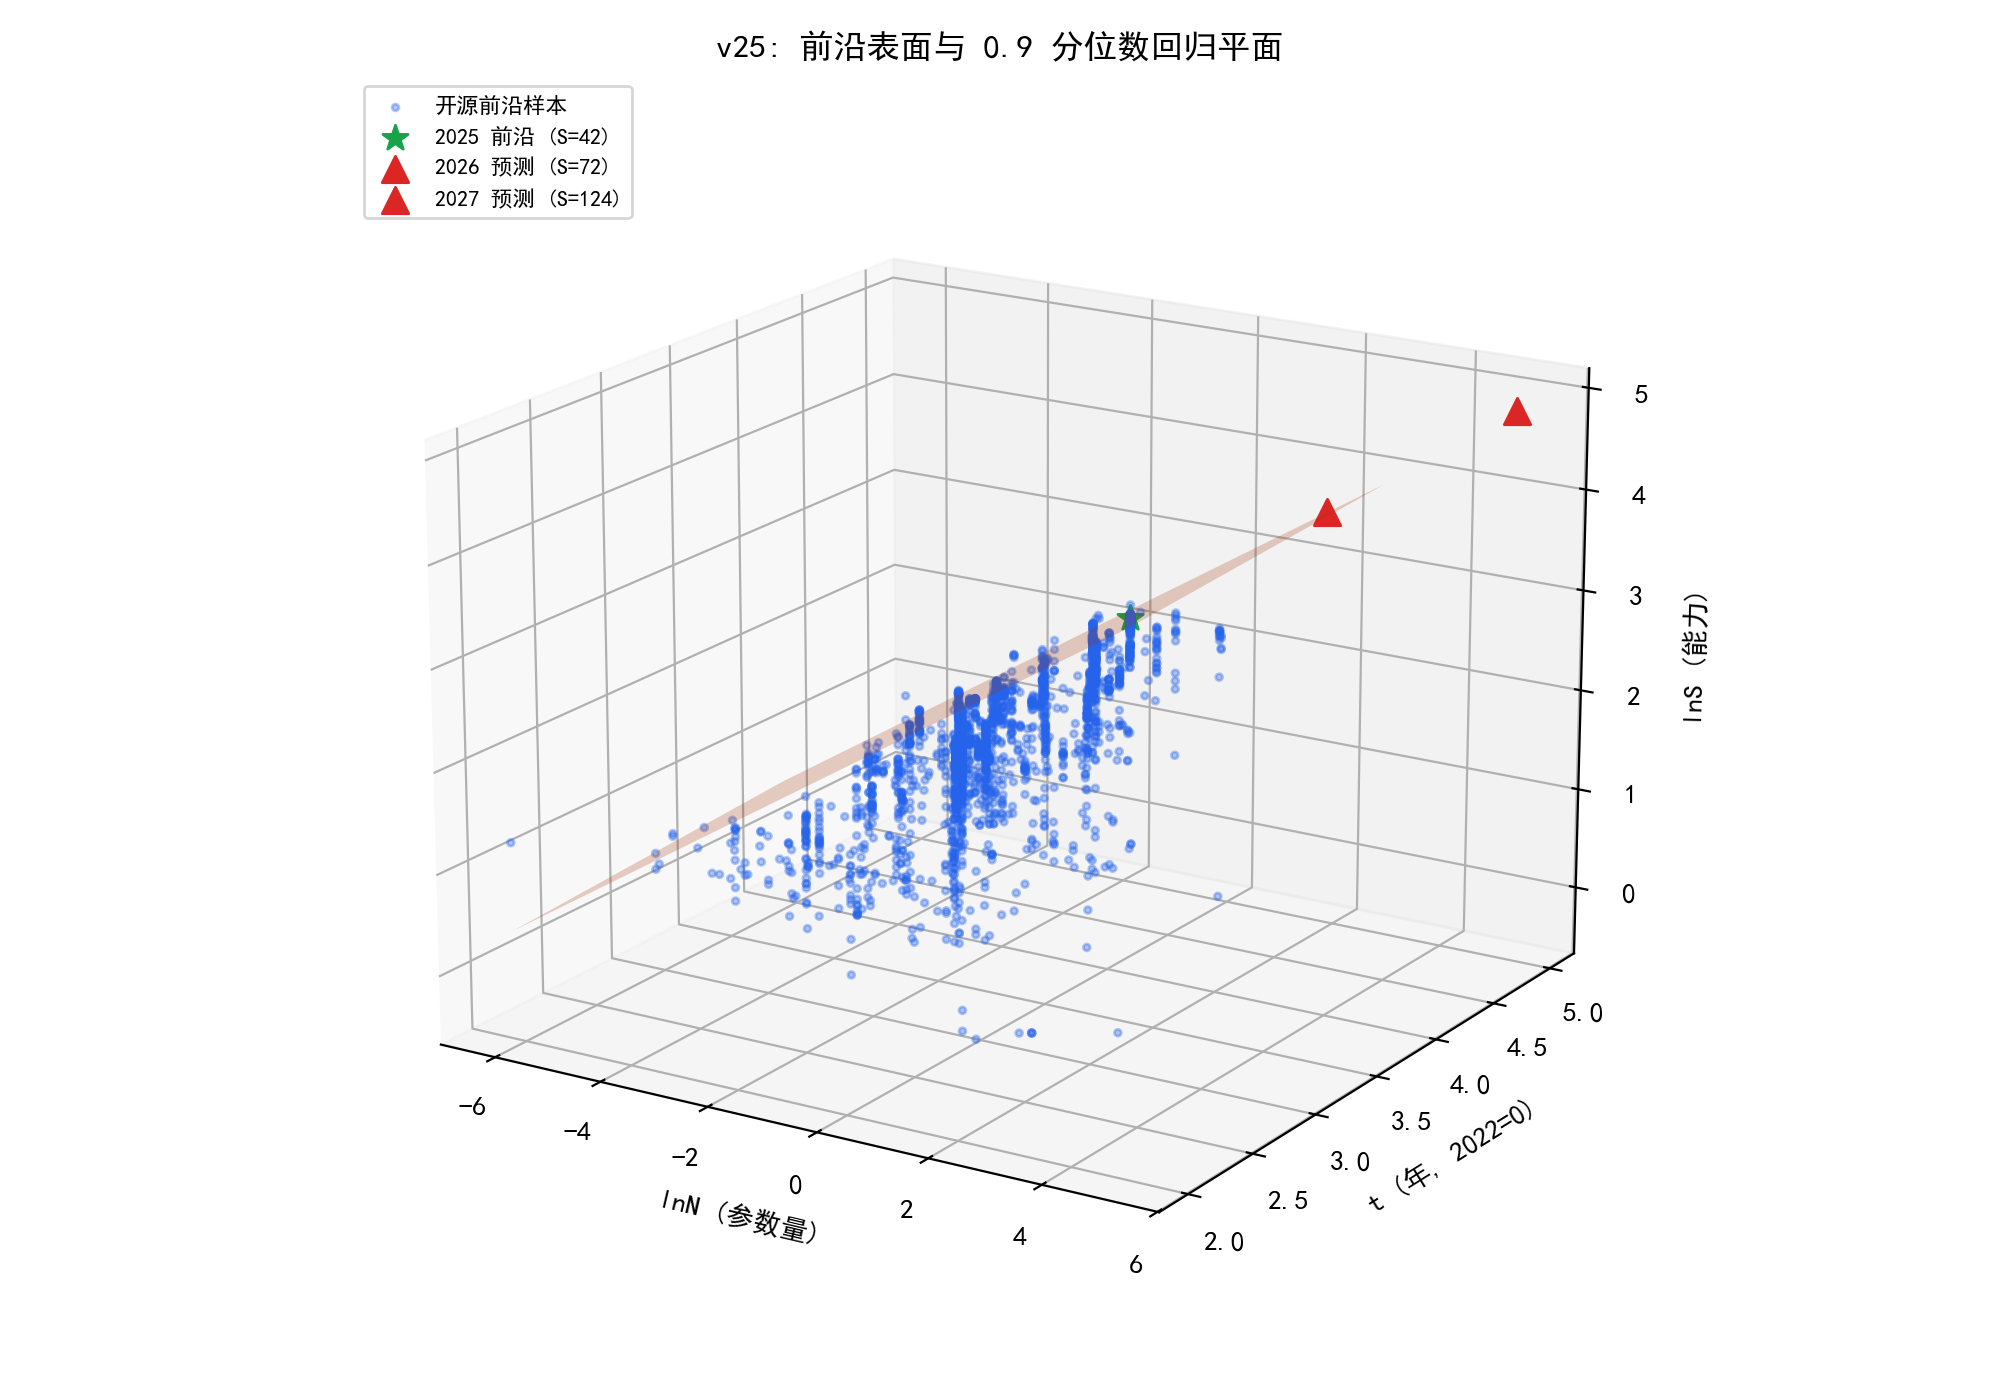
\includegraphics[width=0.88\textwidth]{figures/v25_p4_3d_surface.png}
\caption{能力前沿 3D 表面与 0.9 分位数回归平面（星标=2025 前沿，三角=预测点）。}
\label{fig:p4_3d}
\end{figure}

\textbf{家族留出验证}（图 \ref{fig:p4_familycv}）：把前沿模型按家族分桶
（llama/qwen/gemma/mistral/phi/yi/other 七族；样本 $n=2493$，其中
2484 条归族），逐个
家族留出拟合 $\ln S=c_0+b_N\ln N+b_T t$。全量 OLS 得 $b_N=0.366$
（与 QR90 的 0.364 一致，估计器稳健）；家族留出下 $b_N\in[0.353,0.384]$，
最大偏离约 5\%——\textbf{规模弹性跨家族稳定}，前沿斜率不是由单一家族
驱动。留出残差显示：qwen（+0.223）与 phi（+0.161）显著高于
规模--时间预测线（技术进步更快），llama/mistral 略低于线；留出 $R^2$
中 qwen 最高（0.588），gemma（0.109）与 phi（0.286）最低，说明这两家
族的分数更受个体因素影响。该验证同时说明：`双驱动''模型对领先家族的
``超出规模''能力（如 qwen）存在系统性低估，预测区间已涵盖此差异。

\begin{figure}[htbp]
\centering
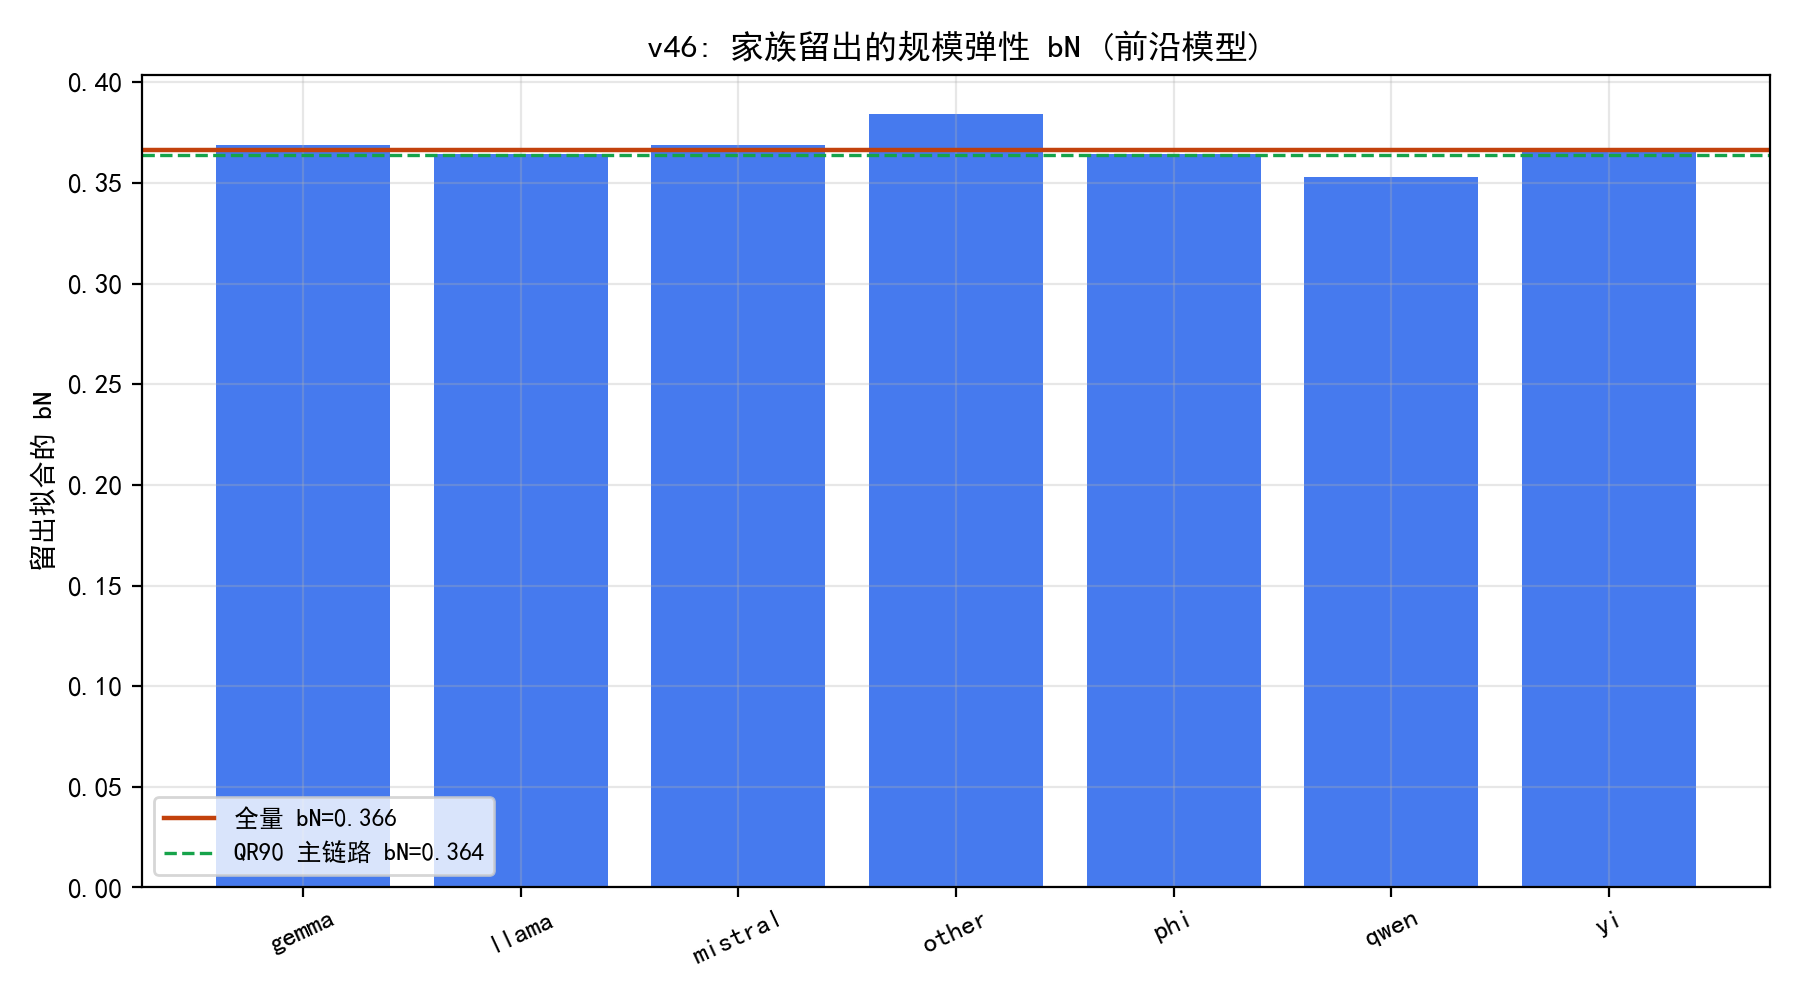
\includegraphics[width=0.8\textwidth]{figures/v46_p4_family_cv.png}
\caption{家族留出的规模弹性 $b_N$：全家族稳定在 0.36 附近。}
\label{fig:p4_familycv}
\end{figure}

\begin{figure}[htbp]
\centering
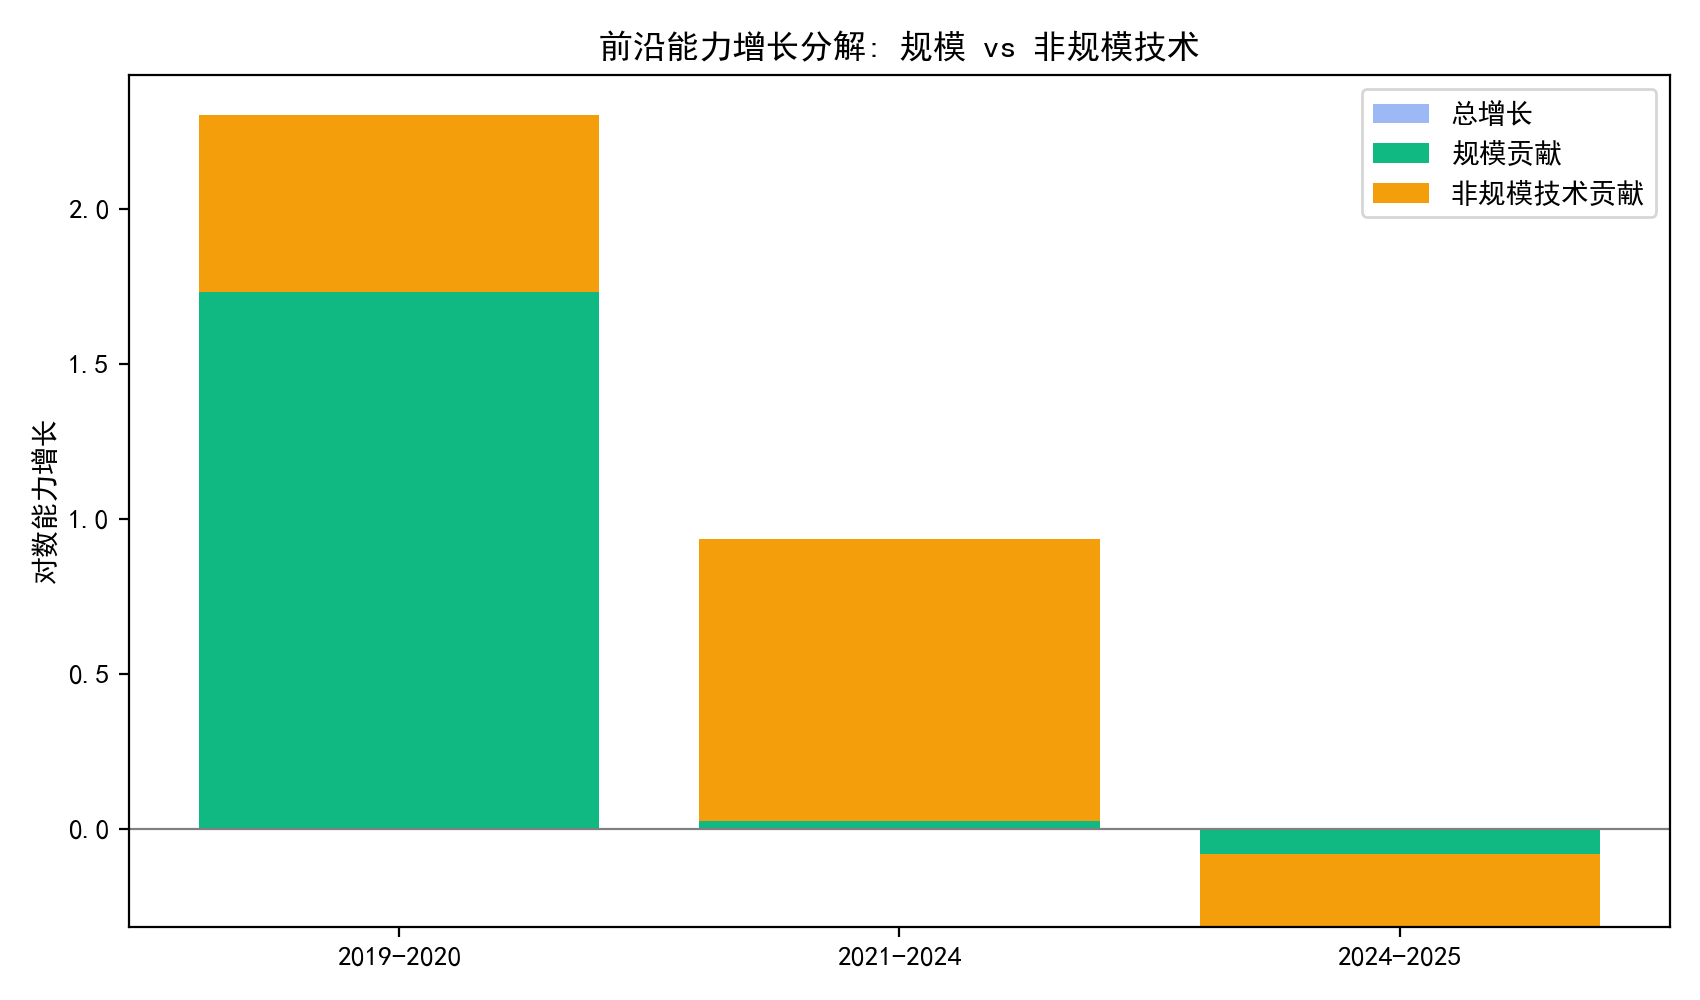
\includegraphics[width=0.8\textwidth]{figures/p4_decomposition.png}
\caption{前沿能力增长分解：规模贡献与非规模技术贡献。}
\label{fig:p4_decomp}
\end{figure}

\subsection{模型验证}

\paragraph{Loss--Benchmark 桥接（C6）}

为统一``损失''与``排行榜分''两套度量，用 C6 的 75 个模型的验证损失与
Benchmark 平均分建立 logit--log 线性映射：
\begin{equation}
\text{logit}\bigl(\tfrac{S}{100}\bigr)=0.852-3.304\ln L,
\qquad R^2=0.276\ (n=75).
\label{eq:bridge}
\end{equation}
映射误差按可比性分组：同一模型同一验证集（High）误差均值 $7.96\pm2.62$
分，不同验证集近似（Medium）为 $-3.13\pm10.26$ 分——说明桥接在中低精度
场景可用，且高可比性样本误差更集中。该桥接可将问题二的损失预测换算为能力
分，实现``资源 $\to$ 损失 $\to$ 能力''的完整链。

\begin{figure}[htbp]
\centering
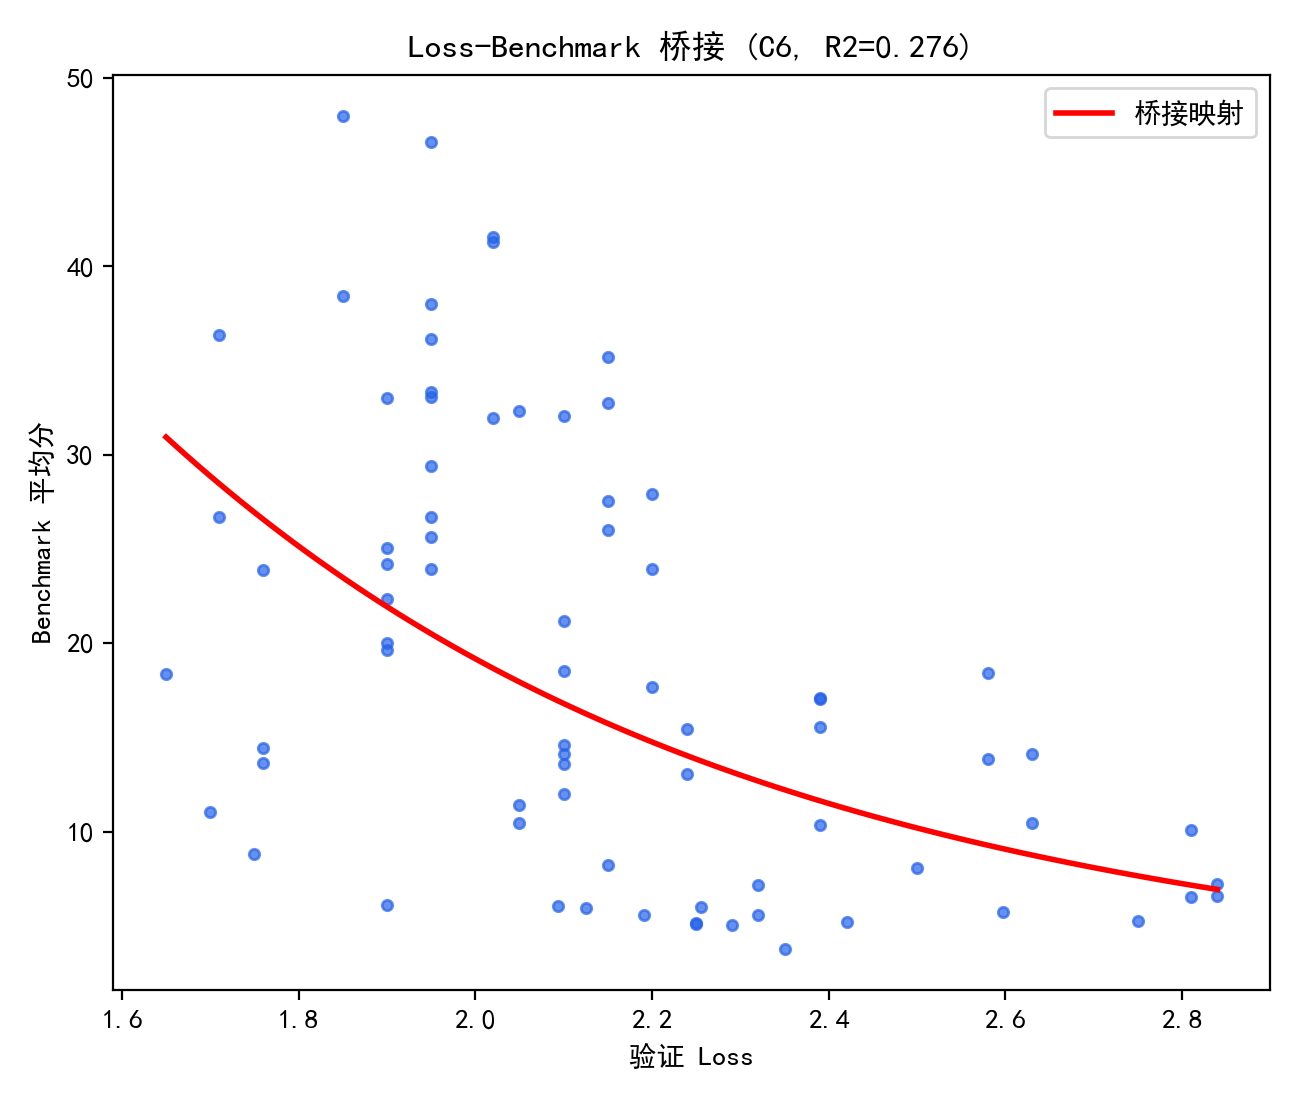
\includegraphics[width=0.62\textwidth]{figures/p4_bridge.png}
\caption{Loss--Benchmark 桥接映射（C6，75 个模型）。}
\label{fig:p4_bridge}
\end{figure}

\paragraph{C8 逐任务聚合分析}

从 C8 的 1863 个模型目录解析全部 JSON（跳过 4 个损坏文件，取每目录最新
记录，得 1860 个模型），提取 6 维逐任务 \texttt{acc}（IFEval 取
\texttt{inst\_level\_strict\_acc}、MATH 取 \texttt{exact\_match}、其余取
\texttt{acc\_norm}），聚合为模型级平均分：

\begin{table}[htbp]
\centering
\caption{C8 逐任务聚合得分（1860 模型）}
\begin{tabular}{c|cccccc}
\toprule
任务 & BBH & IFEval & MUSR & MMLU & GPQA & MATH \\
\midrule
平均 & 0.475 & 0.402 & 0.400 & 0.320 & 0.298 & 0.113 \\
标准差 & 0.116 & 0.215 & 0.046 & 0.130 & 0.039 & 0.120 \\
\bottomrule
\end{tabular}
\end{table}

任务难度排序（MATH 最难、BBH 相对最容易）与常识一致。将 C8 聚合分与 C1
排行榜平均分按模型名归一化匹配（$n=1895$），Spearman 相关 $=0.989$，说明
C8 逐任务明细与 C1 汇总高度一致，聚合口径可靠，可作为排行榜得分的独立
复算验证。同时 BBH/GPQA 等推理任务的内部子任务（如 BBH 的 27 个子任务）
也可逐项提取，用于刻画``推理能力谱''，此处从略。

\begin{figure}[htbp]
\centering
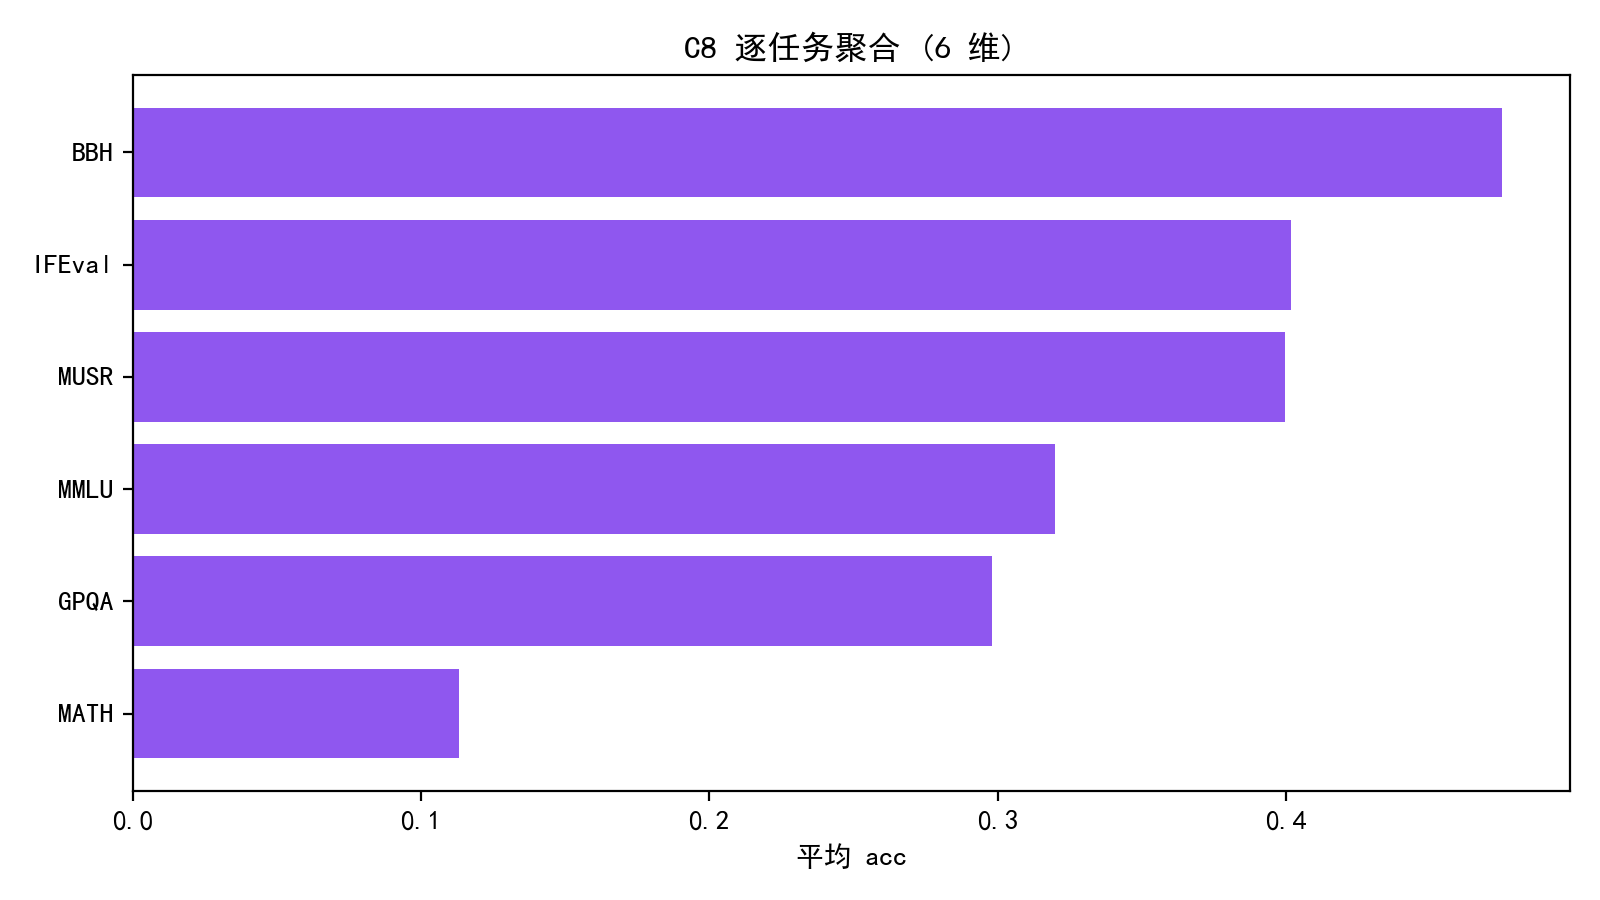
\includegraphics[width=0.7\textwidth]{figures/p4_c8_tasks.png}
\caption{C8 逐任务聚合得分（6 维）。}
\label{fig:p4_c8}
\end{figure}

问题四的验证由三类手段构成：\textbf{可视化验证}（图
\ref{fig:p4_frontier}--\ref{fig:p4_c8} 给出前沿拟合、3D 表面、预测区间与
历史回测）、\textbf{数值交叉验证}（五框架分位数回归系数一致、分位数族
$0.5$--$0.99$ 上规模贡献单调上升且每分位五框架复算一致、历史回测外推与
2024/2025 实际前沿吻合、C8 与 C1 Spearman 0.989）与\textbf{物理/几何规律
对照}（规模--时间等能力线斜率 $-0.245$、能力目标 $\to$ 训练算力 6.6 万
卡天、推理任务增速快于知识任务与文献观察一致）。三项验证均通过，证实了
前沿分解与预测的合理性。

问题四建立了分位数前沿回归 $\ln S=2.481+0.364\ln N+0.089t$，把前沿能力
年增速分解为规模 83.7\% 与非规模 16.3\%；基于 C4 参数增速构建基础与放缓
情景，预测 12/24 个月前沿（基础 71.7/123.9，放缓 57.1/78.6，含 90\% 区间）；
C6 桥接完成损失--能力统一；C8 逐任务聚合与 C1 对照 Spearman 0.989，验证
口径可靠。
